\documentclass[11pt,a4paper]{article}

% définition des marges du document
\setlength{\topmargin}{0cm}
\setlength{\headheight}{0.4cm}
\setlength{\headsep}{0.8cm}
\setlength{\footskip}{1cm}
\setlength{\textwidth}{17cm}
\setlength{\textheight}{25cm}
\setlength{\voffset}{-1.5cm}
\setlength{\hoffset}{-0.5cm}
\setlength{\oddsidemargin}{0cm}
\setlength{\evensidemargin}{0cm}

\usepackage[
        backend=biber,
        style=phys,  
        mcite=true,
        subentry,
        hyperref=true,
        ]{biblatex}
\addbibresource{Rapport.bib}

\usepackage{graphicx} % inclusion des figures
\usepackage{tabularx} % gestion avancée des tableaux

\usepackage{physics}
\usepackage{amsmath} % collection de symboles mathématiques
\usepackage{amssymb} % collection de symboles mathématiques

\usepackage[utf8]{inputenc}
\usepackage[T1]{fontenc}
\DeclareUnicodeCharacter{2212}{-}

\usepackage[english]{babel}

\usepackage{siunitx}
\usepackage[version=4]{mhchem}


\usepackage{xcolor} % gestion de différentes couleurs

\definecolor{linkcolor}{rgb}{0,0,0.6} % définition de la couleur des liens pdf
\newcommand{\titou}[1]{\textcolor{red}{#1}}
\newcommand{\antoine}[1]{\textcolor{orange}{#1}}
\usepackage[ pdftex,colorlinks=true,
pdfstartview=FitV,
linkcolor= linkcolor,
citecolor= linkcolor,
urlcolor= linkcolor,
hyperindex=true,
hyperfigures=false]
{hyperref} % fichiers pdf 'intelligents', avec des liens entre les références, etc.
\usepackage{fancyhdr} % entêtes et pieds de pages personnalisés

% définition de l'entête et du pied de page
\pagestyle{fancy}
\fancyhead[L]{\scriptsize \textsc{Perturbation theory in the complex plane}}
\fancyhead[R]{\scriptsize \textsc{Antoine \textsc{MARIE}}}
\fancyfoot[C]{ \thepage}

\newcommand{\bH}{\mathbf{H}}
\newcommand{\bV}{\mathbf{V}}
\newcommand{\pt}{$\mathcal{PT}$}

\begin{document}

% Pour faciliter la mise en forme de la page du titre, on supprime l'indentation automatique en début de paragraphe
\setlength{\parindent}{0pt}

% Pas d'en-tête ni de pied pour la première page
\thispagestyle{empty}


\includegraphics[height=2cm]{logoens.eps} \hfill 
\includegraphics[height=2cm]{logoucbl.eps} \hfill 
\includegraphics[height=2cm]{logounivlyon.eps}
\vspace{0.5cm}

\begin{tabularx}{\textwidth}{@{} l X l @{} }
{\sc Licence / Master Science de la matière} & & Stage 2019-2020 \\
{\it École Normale Supérieure de Lyon} & & Antoine \textsc{MARIE} \\
{\it Université Claude Bernard Lyon I} & & M1 Chimie
\end{tabularx}

\begin{center}

\vspace{1.5cm}

\rule[11pt]{5cm}{0.5pt}

\textbf{\huge Pertubation theory in the complex plane}

\rule{5cm}{0.5pt}

\vspace{1.5cm}

\parbox{15cm}{\small
\textbf{Abstract} : \it In this work, we explore the extension of quantum chemistry in the complex plane. We observe that the physics of a quantum system is intimately connected to the position of the energy singularities in the complex plane. After a brief presentation of the fundamental notions of quantum chemistry and perturbation theory in the complex plane, we provide a historical overview of the various research activities that have been performed on the physic of singularities. Then we connect and further discuss these different aspects using the spherium model (i.e., two opposite-spin electrons restricted to remain on the surface of a sphere) as a theoretical playground. In particular, we explore various perturbative partitioning strategies and the effects of symmetry breaking on the singularity structure of the electronic energy. This provides fundamental insights on the location of these singularities in the complex plane (that one calls exceptional points) and, specifically, on the magnitude of the radius of convergence associated with the perturbative treatment.
}

\vspace{0.5cm}

\parbox{15cm}{
\textbf{Keywords} : \it quantum chemistry, perturbation theory, complex plane, spherium, exceptional points, radius of convergence, symmetry breaking
} %fin de la commande \parbox des mots clefs

\vspace{0.5cm}

\parbox{15cm}{
Internship supervisor:

{\bf Pierre-François \textsc{LOOS}}

\href{mailto:loos@irsamc.ups-tlse.fr}{\tt loos@irsamc.ups-tlse.fr} / tél. (+33) 5 61 55 73 39

Laboratoire de Chimie et Physique Quantiques

{\it 118, route de Narbonne

31062 Toulouse - France}

\url{https://www.irsamc.ups-tlse.fr/loos}
} %fin de la commande \parbox encadrant / laboratoire d'accueil

\vspace{0.5cm}

\includegraphics[height=2cm]{LCPQ_logo.pdf} \hfill 
\includegraphics[height=2cm]{LogoCNRS.eps} \hfill 
\includegraphics[height=2cm]{UPS_logo.jpg}

\end{center}

\vfill
\hfill \today

\newpage
\thispagestyle{empty}

\setlength{\parindent}{17pt}

\section*{Acknowledgments}

\tableofcontents

\newpage
\setcounter{page}{1}

%============================================================%
\section{Introduction}
%============================================================%

\subsection{Background}

Due to the ubiquitous influence of processes involving electronic excited states in physics, chemistry, and biology, their faithful description from first principles has been one of the grand challenges faced by theoretical chemists since the dawn of computational chemistry. 
Accurately predicting ground- and excited-state energies (hence excitation energies) is particularly valuable in this context, and it has concentrated most of the efforts within the community.
An armada of theoretical and computational methods have been developed to this end, each of them being plagued by its own flaws. 
The fact that none of these methods is successful in every chemical scenario has encouraged chemists to carry on the development of new excited-state methodologies, their main goal being to get the most accurate excitation energies (and properties) at the lowest possible computational cost in the most general context.

One common feature of all these methods is that they rely on the notion of quantised energy levels of Hermitian quantum mechanics, in which the different electronic states of a molecule or an atom are energetically ordered, the lowest being the ground state while the higher ones are excited states. 
Within this quantised paradigm, electronic states look completely disconnected from one another.
Many current methods study excited states using only ground-state information, creating a ground-state bias that leads to incorrect excitation energies.
However, one can gain a different perspective on quantisation extending quantum chemistry into the complex domain.
In a non-Hermitian complex picture, the energy levels are \textit{sheets} of a more complicated topological manifold called \textit{Riemann surface}, and they are smooth and continuous \textit{analytic continuation} of one another.
In other words, our view of the quantised nature of conventional Hermitian quantum mechanics arises only from our limited perception of the more complex and profound structure of its non-Hermitian variant.
The realisation that ground and excited states both emerge from one single mathematical structure with equal importance suggests that excited-state energies can be computed from first principles in their own right.
One could then exploit the structure of these Riemann surfaces to develop methods that directly target excited-state energies without needing ground-state information.

By analytically continuing the electronic energy $E(\lambda)$ in the complex domain (where $\lambda$ is a coupling parameter), the ground and excited states of a molecule can be smoothly connected.
This connection is possible because by extending real numbers to the complex domain, the ordering property of real numbers is lost.
Hence, electronic states can be interchanged away from the real axis since the concept of ground and excited states has been lost.
Amazingly, this smooth and continuous transition from one state to another has recently been experimentally realized in physical settings such as electronics, microwaves, mechanics, acoustics, atomic systems and optics \cite{Bittner_2012, Chong_2011, Chtchelkatchev_2012, Doppler_2016, Guo_2009, Hang_2013, Liertzer_2012, Longhi_2010, Peng_2014, Peng_2014a, Regensburger_2012, Ruter_2010, Schindler_2011, Szameit_2011, Zhao_2010, Zheng_2013, Choi_2018, El-Ganainy_2018}.


Exceptional points (EPs) \cite{Heiss_1990, Heiss_1999, Heiss_2012, Heiss_2016} are non-Hermitian analogs of conical intersections (CIs) \cite{Yarkony_1996} where two states become exactly degenerate.
CIs are ubiquitous in non-adiabatic processes and play a key role in photo-chemical mechanisms.
In the case of auto-ionizing resonances, EPs have a role in deactivation processes similar to CIs in the decay of bound excited states.
Although Hermitian and non-Hermitian Hamiltonians are closely related, the behavior of their eigenvalues near degeneracies is starkly different.
For example, encircling non-Hermitian degeneracies at EPs leads to an interconversion of states, and two loops around the EP are necessary to recover the initial energy (see \autoref{fig:TopologyEP} for a graphical example).
Additionally, the wave function picks up a geometric phase (also known as Berry phase \cite{Berry_1984}) and four loops are required to recover the initial wave function.
In contrast, encircling Hermitian degeneracies at CIs only introduces a geometric phase while leaving the states unchanged.
More dramatically, whilst eigenvectors remain orthogonal at CIs, at non-Hermitian EPs the eigenvectors themselves become equivalent, resulting in a \textit{self-orthogonal} state \cite{MoiseyevBook}.
More importantly here, although EPs usually lie off the real axis, these singular points are intimately related to the convergence properties of perturbative methods and avoided crossing on the real axis are indicative of singularities in the complex plane \cite{Olsen_1996, Olsen_2000}.

\begin{figure}[h!]
    \centering
    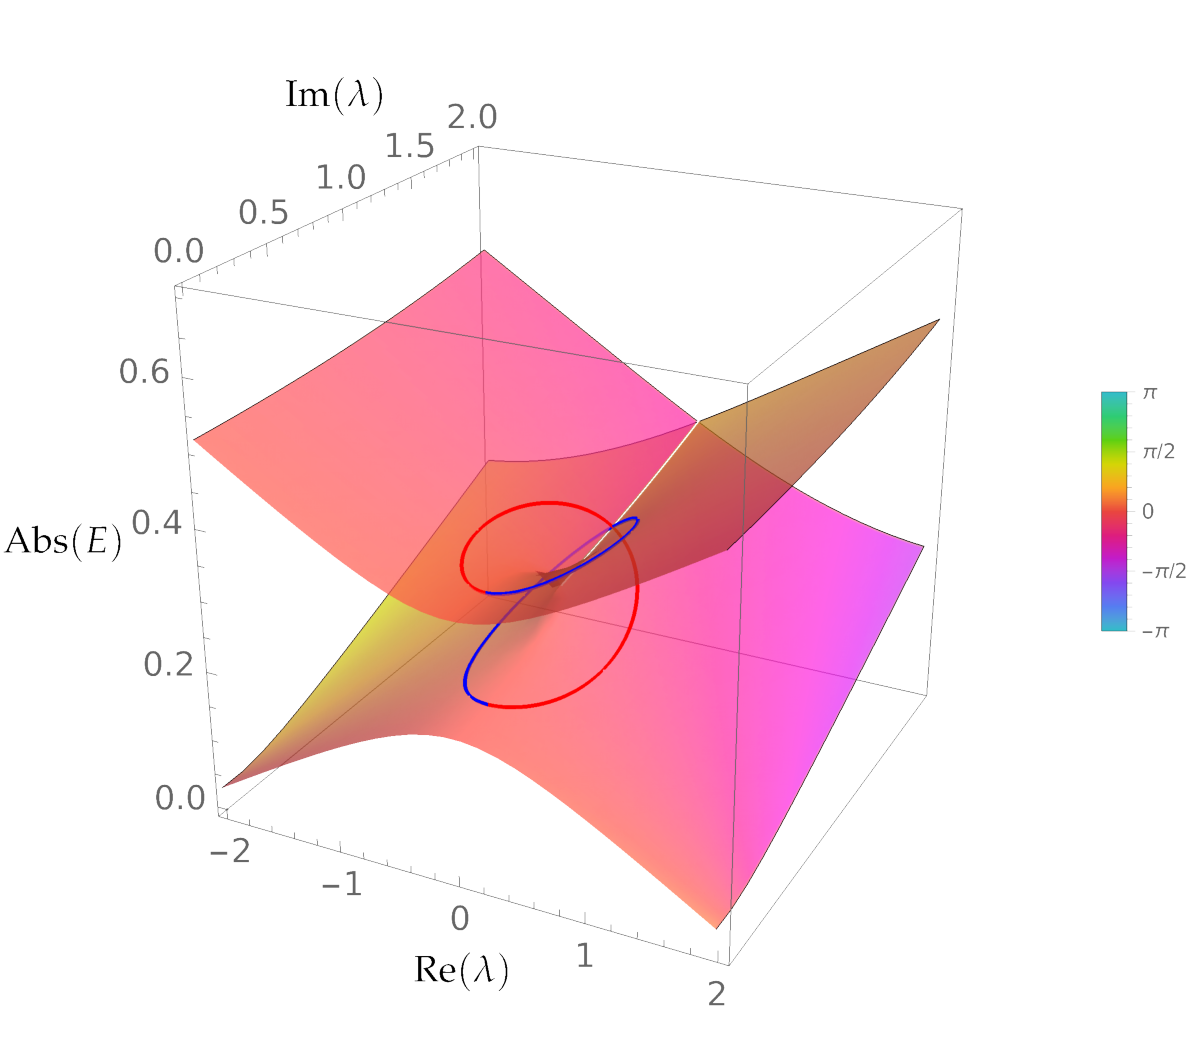
\includegraphics[width=0.7\textwidth]{TopologyEP.pdf}
    \caption{\centering A generic EP with the square root branch point topology. A loop around the EP interconvert the states.}
    \label{fig:TopologyEP}
\end{figure}

\subsection{An illustrative example}
In order to highlight the general properties of EPs mentioned above, we propose to consider the following $2 \times 2$ Hamiltonian commonly used in quantum chemistry

\begin{equation}
\label{eq:H_2x2}
	\bH = 
	\begin{pmatrix}
		\epsilon_1	&	\lambda	\\
		\lambda		&	\epsilon_2
	\end{pmatrix},
\end{equation}
which represents two states of energies $\epsilon_1$ and $\epsilon_2$ coupled with a strength of magnitude $\lambda$.
This Hamiltonian could represent, for example, a minimal-basis configuration interaction with doubles (CID) for the hydrogen molecule \cite{SzaboBook}.

\begin{figure}[h!]
    \centering
    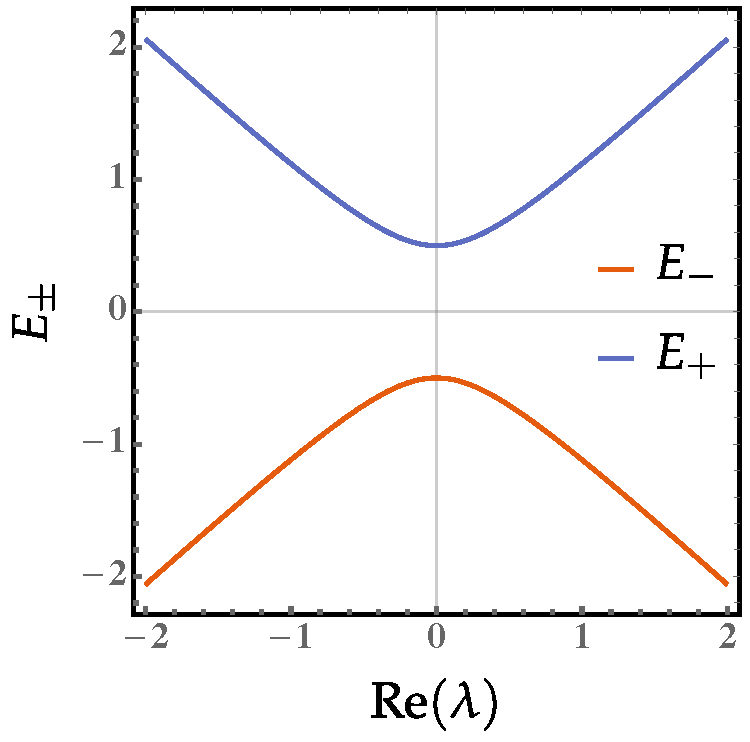
\includegraphics[width=0.45\textwidth]{2x2.pdf}
    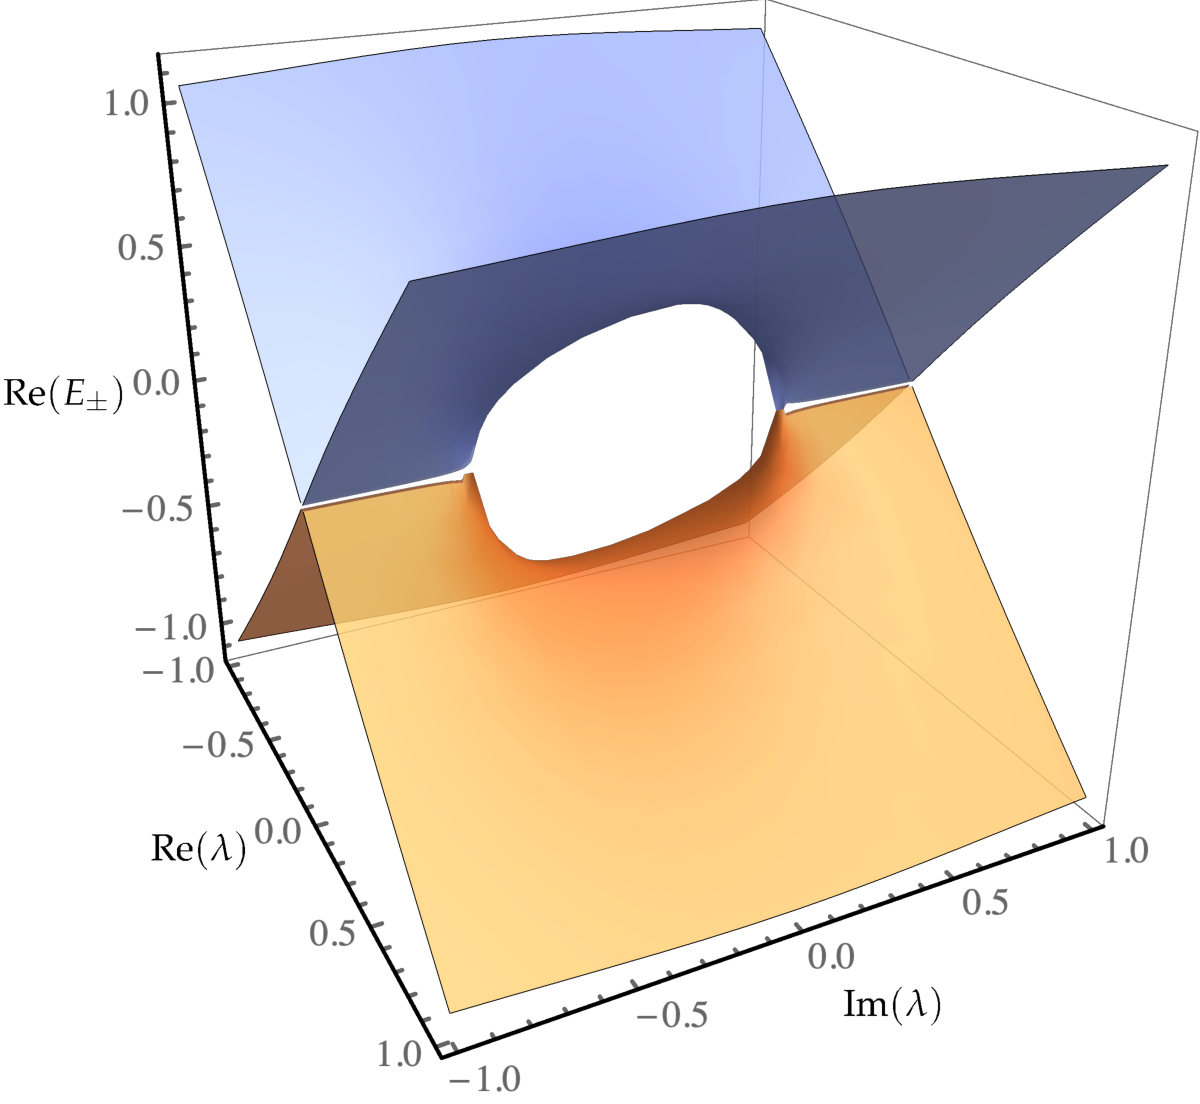
\includegraphics[width=0.45\textwidth]{i2x2.pdf}
    \caption{\centering Energies, as given by Eq.~\eqref{eq:E_2x2}, of the Hamiltonian \eqref{eq:H_2x2} as a function of $\lambda$ with $\epsilon_1 = -1/2$ and $\epsilon_2 = +1/2$.}
    \label{fig:2x2}
\end{figure}

For real $\lambda$, the Hamiltonian \eqref{eq:H_2x2} is clearly Hermitian, and it becomes non-Hermitian for any complex $\lambda$ value.
Its eigenvalues are
\begin{equation}
\label{eq:E_2x2}
	E_{\pm} = \frac{\epsilon_1 + \epsilon_2}{2} \pm \frac{1}{2} \sqrt{(\epsilon_1 - \epsilon_2)^2 + 4\lambda^2},
\end{equation}
and they are represented as a function of $\lambda$ in Fig.~\ref{fig:2x2}.
One notices that the two states become degenerate only for a pair of complex conjugate values of $\lambda$
\begin{equation}
\label{eq:lambda_EP}
	\lambda_\text{EP} = \pm i\,\frac{\epsilon_1 - \epsilon_2}{2},
	\quad
	\text{with energy}	
	\quad
	E_\text{EP} = \frac{\epsilon_1 + \epsilon_2}{2},
\end{equation}
which correspond to square-root singularities in the complex-$\lambda$ plane (see \autoref{fig:2x2}).
These two $\lambda$ values, given by Eq.~\eqref{eq:lambda_EP}, are the so-called EPs and one can clearly see that they connect the ground and excited states.
Starting from $\lambda_\text{EP}$, two square-root branch cuts run on the imaginary axis towards $\pm i \infty$.
In the real $\lambda$ axis, the point for which the states are the closest ($\lambda = 0$) is called an avoided crossing and this occurs at $\lambda = \Re(\lambda_\text{EP})$.
The ``shape'' of the avoided crossing is linked to the magnitude of $\Im(\lambda_\text{EP})$: the smaller $\Im(\lambda_\text{EP})$, the sharper the avoided crossing is.

Around $\lambda = \lambda_\text{EP}$, Eq.~\eqref{eq:E_2x2} behaves as \cite{MoiseyevBook}
\begin{equation} \label{eq:E_EP}
        E_{\pm} = E_\text{EP} \pm \sqrt{2\lambda_\text{EP}} \sqrt{\lambda - \lambda_\text{EP}},
\end{equation}
and following a complex contour around the EP, i.e.~$\lambda = \lambda_\text{EP} + R \exp(i\theta)$, yields
\begin{equation}
        E_{\pm}(\theta) = E_\text{EP} \pm \sqrt{2\lambda_\text{EP} R}  \exp(i\theta/2),
\end{equation}
and we have
\begin{align}
	E_{\pm}(2\pi) & = E_{\mp}(0),
	&
	E_{\pm}(4\pi) & = E_{\pm}(0).
\end{align}
This evidences that encircling non-Hermitian degeneracies at EPs leads to an interconversion of states, and two loops around the EP are necessary to recover the initial energy.

The eigenvectors associated to the eigenenergies \eqref{eq:E_2x2} are
\begin{equation}\label{eq:phi_2x2}
\phi_{\pm}=\begin{pmatrix}
(\epsilon_1 - \epsilon_2 \pm \sqrt{(\epsilon_1 - \epsilon_2)^2 + 4\lambda^2})/2\lambda \\ 1
\end{pmatrix},
\end{equation}
and, for $\lambda=\lambda_\text{EP}$, they become
\begin{align}
	\phi_{\pm}(i\,\frac{\epsilon_1 - \epsilon_2}{2}) & = \begin{pmatrix} -i \\ 1\end{pmatrix},
	&
	\phi_{\pm}(-i\,\frac{\epsilon_1 - \epsilon_2}{2}) & = \begin{pmatrix} i \\ 1\end{pmatrix}.
\end{align}
which are self-orthogonal i.e. their norm is equal to zero. 
Using Eq.~\eqref{eq:E_EP}, Eq.~\eqref{eq:phi_2x2} can be recast as
\begin{equation}\label{eq:phi_EP}
\phi_{\pm}=
	\begin{pmatrix}
		(\epsilon_1-\epsilon_2)/2\lambda \pm \sqrt{2\lambda_\text{EP}} \sqrt{\lambda - \lambda_\text{EP}}/\lambda 
		\\ 
		1
	\end{pmatrix}.
\end{equation}
We have seen that the EP inherits its topology from the double valued function $\sqrt{\lambda - \lambda_\text{EP}}$. Then if the eigenvectors are normalised they behave as $(\lambda - \lambda_\text{EP})^{-1/4}$ which gives the following pattern when looping around one EP:
\begin{align}
	\phi_{\pm}(2\pi) & = \phi_{\mp}(0),
	&
	\phi_{\pm}(4\pi) & = -\phi_{\pm}(0) \\
	\phi_{\pm}(6\pi) & = -\phi_{\mp}(0),
	&
	\phi_{\pm}(8\pi) & = \phi_{\pm}(0).
\end{align}
In plain words, four loops around the EP are necessary to recover the initial state. 
We can also see that looping the other way around leads to a different pattern.
\antoine{Is this a bit better like this ?}

%============================================================%
\section{Perturbation theory}
%============================================================%

\subsection{Rayleigh-Schr\"odinger perturbation theory}

Within (time-independent) Rayleigh-Schr\"odinger perturbation theory, the Schr\"odinger equation 
\begin{equation} \label{eq:SchrEq}
	\bH \Psi = E \Psi
\end{equation} 
is recast as 
\begin{equation} \label{eq:SchrEq-PT}
	\bH(\lambda) \Psi(\lambda) = (\bH^{(0)} + \lambda \bV ) \Psi(\lambda) = E(\lambda) \Psi(\lambda),
\end{equation}
where $\bH^{(0)}$ is the zeroth-order Hamiltonian and $\bV = \bH - \bH^{(0)}$ is the so-called perturbation.
The ``physical'' system of interest is recovered by setting the coupling parameter $\lambda$ to unity.
This decomposition is obviously non-unique and motivated by several factors as discussed below.

Accordingly to Eq.~\eqref{eq:SchrEq-PT}, the energy can then be written as a power series of $\lambda$
\begin{equation} \label{eq:Elambda}
	E(\lambda) = \sum_{k=0}^\infty \lambda^k E^{(k)}
\end{equation}
However it is not guaranteed that the series \eqref{eq:Elambda} has a radius of convergence $\abs{\lambda_0} < 1$. 
In other words, the series might well be divergent for the physical system at $\lambda = 1$. 
One can prove that the actual value of the radius of convergence $\abs{\lambda_0}$ can be obtained by looking for the singularities of $E(\lambda)$ in the complex $\lambda$ plane.
This is due to the following theorem \cite{Goodson_2012}: 
\begin{quote}
	\textit{``The Taylor series about a point $z_0$ of a function over the complex $z$ plane will converge at a value $z_1$ if the function is non-singular at all values of $z$ in the circular region centered at $z_0$ with radius $\abs{z_1 − z_0}$. If the function has a singular point $z_s$ such that $\abs{z_s − z_0} < \abs{z_1 − z_0}$, then the series will diverge when evaluated at $z_1$.''}
\end{quote}
This theorem means that the radius of convergence of the perturbation series is equal to the distance to the origin of the closest singularity of $E(\lambda)$. To illustrate this result we  consider the simple function \eqref{eq:DivExample}. This function is smooth for $x \in \mathbb{R}$ and infinitely differentiable in $\mathbb{R}$. One would expect that the Taylor series of such a function would be convergent for all $x \in \mathbb{R}$, however this series is divergent for $x\geq1$. This is because the function has four singularities in the complex plane ($x = e^{i\pi/4}, e^{-i\pi/4}, e^{i3\pi/4}, e^{-i3\pi/4}$) with a modulus equal to 1. This simple example shows the importance of the singularities in the complex plane to understand the convergence properties on the real axis.

\begin{equation} \label{eq:DivExample}
f(x)=\frac{1}{1+x^4}
\end{equation}

\subsection{The Hartree-Fock Hamiltonian}

In the Born-Oppenheimer approximation, the equation \eqref{eq:ExactHamiltonian} gives the exact electronic Hamiltonian for a chemical system with $n$ electrons and $N$ nuclei. The first term is the kinetic energy of the electrons, the two following terms account respectively for the electron-nuclei attraction and the electron-electron repulsion.

\begin{equation}\label{eq:ExactHamiltonian}
    \bH=\sum\limits_{i=1}^{n}\left[ -\frac{1}{2}\grad_i^2 - \sum\limits_{k=1}^{N} \frac{Z_k}{|\vb{r}_i-\vb{R}_k|}+\sum\limits_{i<j}^{n}\frac{1}{|\vb{r}_i-\vb{r}_j|}\right]
\end{equation}

In the Hartree-Fock (HF) approximation the wave function is approximated as a single Slater determinant (which is an anti-symmetric combination of $n$ one electron spin-orbitals). Rather than solving the equation \eqref{eq:SchrEq}, the Hartree-Fock theory uses the variational principle to find an approximation to $\Psi$. Hence the Slater determinants are not eigenfuctions of the exact Hamiltonian $\bH$. However, they are eigenfunctions of an approximated Hamiltonian $\bH^{(0)}$, called the Hartree-Fock Hamiltonian, which is the sum of the one-electron Fock operators.

\begin{equation}\label{eq:HFHamiltonian}
\bH^{(0)}= \sum\limits_{i=1}^{n} f(i)
\end{equation}

The eigenfunctions of $f(i)$ are the one-electron spin-orbitals $\phi_a(i)$ used to create the $n$-electron Slater determinant. The equation \eqref{eq:FockOp} gives the eigenvalue equation for the one-electron Fock operator associated with the electron 1. The one-electron core Hamiltonian $h(i)$ are the sum of the kinetic energy of the electron $i$ and the attraction of the nuclei on this electron. The two other terms are the the Coulomb $J_a(i)$ and Exchange $K_a(i)$ operators. Their action on the spin-orbitals are given by the equation \eqref{eq:CoulOp} and \eqref{eq:ExcOp}. The integration is over the spatial and spin coordinates.

\begin{equation}\label{eq:FockOp}
f(1)\phi_a(1) = \left[h(1) + \sum\limits_{b=1}^{n} J_b(1) - K_b(1)\right]\phi_a(1)=\epsilon_a\phi_a(1)
\end{equation}

\begin{equation}\label{eq:CoulOp}
J_b(1)\phi_a(1)=\left[\int\dd\vb{x}_2\phi_b^*(2)\frac{1}{r_{12}}\phi_b(2) \right]\phi_a(1)
\end{equation}

\begin{equation}\label{eq:ExcOp}
K_b(1)\phi_a(1)=\left[\int\dd\vb{x}_2\phi_b^*(2)\frac{1}{r_{12}}\phi_a(2) \right]\phi_b(1)
\end{equation}


\subsection{M{\o}ller-Plesset perturbation theory}

The Hartree-Fock Hamiltonian \eqref{eq:HFHamiltonian} can be used as the zeroth-order Hamiltonian of the equation \eqref{eq:SchrEq-PT}. This partitioning of the Hamiltonian leads to the so-called M{\o}ller-Plesset (MP) perturbation theory \cite{Moller_1934}. The discovery of a partitioning of the Hamiltonian that allowed chemists to recover a part of the correlation energy (i.e. the difference between the exact energy and the Hartree-Fock energy) using perturbation theory has been a major step in the development of post-Hartree-Fock methods. This yields the Hamiltonian $\bH(\lambda)$ of the equation \eqref{eq:MPHamiltonian} where the two-electron part of the Fock operator $f(i)$ has been written $V_i^{HF}$ for convenience.

\begin{equation}\label{eq:MPHamiltonian}
    \bH(\lambda)=\sum\limits_{i=1}^{n}\left[-\frac{1}{2}\grad_i^2 - \sum\limits_{k=1}^{N} \frac{Z_k}{|\vb{r}_i-\vb{R}_k|} + (1-\lambda)V_i^{\text{HF}}+\lambda\sum\limits_{i<j}^{n}\frac{1}{|\vb{r}_i-\vb{r}_j|} \right]
\end{equation}

In the perturbation theory the energy is a power series of $\lambda$ and the physical energy is obtained by taking $\lambda$ equal to 1. We will refer to the energy up to the $n$-th order as the MP$n$ energy. The MP0 energy overestimates the energy by double counting the electron-electron interaction, the MP1 corrects this effect and the MP1 energy is equal to the Hartree-Fock energy. The MP2 energy starts to recover a part of the correlation energy \cite{SzaboBook}.

\begin{equation}
E_{\text{MP}_{n}}= \sum_{k=0}^n E^{(k)}
\end{equation}

But as mentioned before \textit{a priori} there are no reasons that $E_{\text{MP}_{n}}$ is always convergent when $n$ goes to infinity. In fact, it is known that when the Hartree-Fock wave function is a bad approximation of the exact wave function, for example for multi-reference states, the MP method will give bad results \cite{Gill_1986, Gill_1988, Handy_1985, Lepetit_1988}. A smart way to investigate the convergence properties of the MP series is to transform the coupling parameter $\lambda$ into a complex variable. By doing so the Hamiltonian and the energy become functions of this variable. The energy becomes a multivalued function on $n$ Riemann sheets. As mentioned above by searching the singularities of the function $E(\lambda)$ we can get information on the convergence properties of the MP perturbation theory. Those singularities of the energy are exactly the exceptional points connecting the electronic states mentioned in the introduction. The direct computation of the terms of the series is quite easy up to the 4th order and the 5th and 6th order can be obtained at high cost \cite{JensenBook}. But to deeply understand the behavior of the MP series and how it is connected to the singularities, we need to have access to high order terms of the series. For small systems we can have access to the whole series using Full Configuration Interaction (FCI). If the Hamiltonian $H(\lambda)$ is diagonalized in the FCI basis set we get the exact energies (in this finite basis set) and expanding in $\lambda$ allows to to get the MP perturbation series at every order.

\subsection{Alternative partitioning}\label{sec:AlterPart}

The MP partitioning is not the only one possible in electronic structure theory. An other possibility, even more natural than the MP one, is to take the diagonal elements of $\bH$ as the zeroth-order Hamiltonian. Hence, the off-diagonal elements of $\bH(\lambda)$ are the perturbation operator. This partitioning leads to the Epstein-Nesbet (EN) perturbation theory. The zeroth-order eigenstates for this partitioning are Slater determinants as for the MP partitioning. The expression of the second order correction to the energy is given for both MP and EN. The energies at the MP denominator are the orbitals energies whereas in the EN case it is the excitation energies. The i,j indices represent the occupied orbitals and a,b the virtual orbitals of the basis sets.

\begin{equation}\label{eq:EMP2}
E_{\text{MP2}}=\sum\limits_{\substack{i<j \\ a<b}}^{n}\frac{\abs{\mel{ij}{}{ab}}^2}{\epsilon_i + \epsilon_j - \epsilon_a - \epsilon_b}
\end{equation}
\begin{equation}\label{eq:EEN2}
E_{\text{EN2}}=\sum\limits_{\substack{i<j \\ a<b}}^{n}\frac{\abs{\mel{ij}{}{ab}}^2}{}
\end{equation}
where $J_{ij}$ is the matrix element of the Coulomb operator \eqref{eq:CoulOp} and with
\begin{equation}
	\mel{ij}{}{ab}=\braket{ij}{ab} - \braket{ij}{ba}
\end{equation}
where $\braket{ij}{ab}$ is the two-electron integral
\begin{equation}
\braket{ij}{ab}=\int \dd\vb{x}_1\dd\vb{x}_2\phi_i^*(\vb{x}_1)\phi_j^*(\vb{x}_2)r_{12}^{-1}\phi_a(\vb{x}_1)\phi_b(\vb{x}_2)
\end{equation}

Additionally, we will consider two other partitioning. The electronic Hamiltonian can be separated in a one-electron part and in a two-electron part as seen previously. We can use this separation to create two other partitioning:

\begin{itemize}
\item The Weak Correlation partitioning in which the one-electron part is consider as the unperturbed Hamiltonian $\bH^{(0)}$ and the two-electron part is the perturbation operator $\bV$.
\item The Strong Coupling partitioning where the two operators are inverted compared to the weak correlation partitioning.
\end{itemize}

%============================================================%
\section{Historical overview}
%============================================================%

\subsection{Behavior of the M{\o}ller-Plesset series}

When one relies on MP perturbation theory (and more generally on any perturbative partitioning), it would be reasonable to ask for a systematic improvement of the energy with respect to the perturbative order, i.e., one would expect that the more terms of the perturbative series one has, the closer the result from the exact energy.
%In other words, each time a higher-order term is computed, one would like to obtained an overall result closer to the exact energy. 
In other words, one would like a monotonic convergence of the MP series. Assuming this, the only limiting process to get the exact correlation energy (in a finite basis set) would be our ability to compute the terms of this perturbation series.
Unfortunately this is not as easy as one might think because i) the terms of the perturbative series become rapidly computationally cumbersome, and ii) erratic behavior of the perturbative coefficients are not uncommon. For example, in the late 80's, Gill and Radom reported deceptive and slow convergences in stretch systems \cite{Gill_1986, Gill_1988} (see also Refs.~\cite{Handy_1985, Lepetit_1988}). 
In \autoref{fig:RUMP_Gill}, which has been extracted from Ref.~\cite{Gill_1986}, one can see that the restricted MP series is convergent, yet oscillating which is far from being convenient if one is only able to compute the first few terms of the expansion (for example here RMP5 is worse than RMP4). 
On the other hand, the unrestricted MP series is monotonically convergent (except for the first few orders) but very slowly so one cannot use it in practice for systems where one can only compute the first terms.

\begin{figure}[h!]
    \centering
    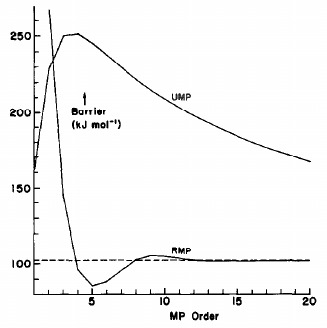
\includegraphics[width=0.45\textwidth]{gill1986.png}
    \caption{\centering Barriers to homolytic fission of \ce{He2^2+} at MPn/STO-3G level ($n = 1$--$20$) (taken from \cite{Gill_1986}).}
    \label{fig:RUMP_Gill}
\end{figure}

When a bond is stretched the exact wave function becomes more and more multi-reference. Yet the HF wave function is restricted to be single Slater determinant.
Thus, it is inappropriate to model (even qualitatively) stretched system. Nevertheless, the HF wave function can undergo a symmetry breaking to lower its energy by sacrificing one of the symmetry of the exact wave function during the process (see for example the case of \ce{H_2} in Ref.~\cite{SzaboBook}). \antoine{It could be expected that  the restricted MP series has inappropriate convergence properties as a restricted HF Slater determinant is a poor approximation of the exact wave function for stretched system. However even in the unrestricted formalism the series does not give accurate results at low orders. Whereas the unrestricted formalism allows a better description of a stretched system because the spatial orbitals of electrons $\alpha$ and $\beta$ are not restricted to be the same \cite{Fukutome_1981}.} Even with this improvement of the zeroth-order wave function the series does not have the smooth and rapidly converging behavior wanted. 

\begin{table}[h!]
    \centering
    \caption{\centering Percentage of electron correlation energy recovered and $\expval{S^2}$ for the \ce{H2} molecule as a function of bond length (r,\si{\angstrom}) in the STO-3G basis set (taken from \cite{Gill_1988}).}
    \begin{tabular}{ccccccc}
\hline
\hline
 $r$ & UHF & UMP2 & UMP3 & UMP4 & $\expval{S^2}$ \\
\hline
0.75 & 0.0\% & 63.8\% & 87.4\% & 95.9\% & 0.00\\
1.35 & 0.0\% & 15.2\% & 26.1\% & 34.9\% & 0.49\\
2.00 & 0.0\% & 01.0\% & 01.8\% & 02.6\% & 0.95\\
2.50 & 0.0\% & 00.1\% & 00.3\% & 00.4\% & 0.99\\
\hline
\hline
\end{tabular}
    \label{tab:SpinContamination}
\end{table}

In the unrestricted framework the singlet ground state wave function is allowed to mix with triplet wave function which leads to spin contamination. Gill \textit{et al.}~highlighted the link between slow convergence of the unrestricted MP series and spin contamination of the wave function as shown in the \autoref{tab:SpinContamination} in the example of \ce{H_2} in a minimal basis \cite{Gill_1988}. 
Handy and coworkers exhibited the same behavior of the series (oscillating and monotonically slowly) in stretched \ce{H_2O} and \ce{NH_2} systems \cite{Handy_1985}. Lepetit et al.~analyzed the difference between the MP and EN partitioning for the unrestricted HF reference \cite{Lepetit_1988}. They concluded that the slow convergence is due to the coupling of the singly and doubly excited configurations. Moreover, the MP and EN numerators in Eqs.~\eqref{eq:EMP2} and \eqref{eq:EEN2} are the same and they vanish when the bond length $r$ goes to infinity. Yet the MP denominators tends towards a constant when $r \to \infty$ so the terms vanish, whereas the EN denominators tends to zero which improves the convergence but can also make the series diverge.
Cremer and He analyzed 29 atomic and molecular systems at the FCI level \cite{Cremer_1996} and regrouped all of these systems in two classes. The class A systems where one observes a monotonic convergence to the FCI energy and the class B for which convergence is erratic after initial oscillations. The sample of systems contains stretched molecules as well as molecules at their equilibrium geometry for various basis sets. They highlighted that \cite{Cremer_1996}
\begin{quote}
	\textit{``Class A systems are characterized by electronic structures with well-separated electron pairs while class B systems are characterized by electronic structures with electron clustering in one or more regions.''}
\end{quote}
They proved that using different extrapolation formulas of the first terms of the MP series for class A and class B systems, this improves the precision of those formulas. The mean deviation from FCI correlation energies is $0.3$ millihartree whereas with the formula that do not distinguish the system it is 12 millihartree. Even if there were still shaded areas and that this classification was incomplete, this work showed that understanding the origin of the different modes of convergence would lead to a more rationalized use of the MP perturbation theory and to more accurate correlation energies.

\subsection{Cases of divergence}

In the late 90's, Olsen \textit{et al.}~have discovered an even more preoccupying behavior of the MP series \cite{}. They showed that the series could be divergent even in systems that they considered as well understood like \ce{Ne} and \ce{HF} (see \autoref{fig:NeHFDiv}) \cite{Olsen_1996, Christiansen_1996}. Cremer and He had already studied these two systems and classified them as ``class B'' systems. However, the analysis of Olsen and coworkers was performed in larger basis sets containing diffuse functions. In these basis sets, they found that the series become divergent at (very) high order.

\begin{figure}[h!]
    \centering
    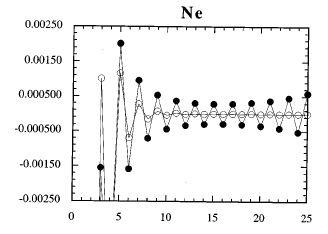
\includegraphics[width=0.45\textwidth]{Nedivergence.png}
    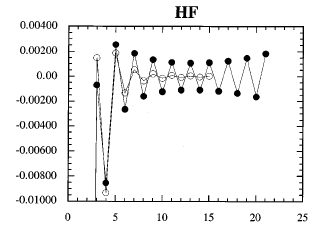
\includegraphics[width=0.45\textwidth]{HFdivergence.png}
    \caption{\centering Correlation contributions for \ce{Ne} and \ce{HF} in the cc-pVTZ-(f/d) $\circ$ and aug-cc-pVDZ $\bullet$ basis sets (taken from \cite{Olsen_1996}).}
    \label{fig:NeHFDiv}
\end{figure}

The discovery of this divergent behavior is worrying as in order to get meaningful and accurate energies, calculations must be performed in large basis sets (as close as possible from the complete basis set limit). Including diffuse functions is particularly important for the case of anions and/or Rydberg excited states where the wave function is much more diffuse than the ground-state one. As a consequence, they investigated further the causes of these divergences as well as the reasons of the different types of convergence. To do so, they analyzed the relation between the dominant singularity (i.e., the closest singularity to the origin) and the convergence behavior of the series \cite{Olsen_2000}. Their analysis is based on Darboux's theorem: 
\begin{quote}
	\textit{``In the limit of large order, the series coefficients become equivalent to the Taylor series coefficients of the singularity closest to the origin. Following the result of this theorem, the convergence patterns of the MP series can be explained by looking at the dominant singularity.''}
\end{quote}

A singularity in the unit circle is designated as an intruder state, more precisely as a front-door (respectively back-door) intruder state if the real part of the singularity is positive (respectively negative). Theie method consists in performing a scan of the real axis to detect the avoided crossing responsible for the pair of dominant singularity. Then by modeling this avoided crossing via a two-state Hamiltonian one can get an approximation of the dominant conjugate pair of singularity by finding the EPs of the $2\times2$ Hamiltonian. The diagonal matrix is the unperturbed Hamiltonian and the other matrix is the perturbative part of the Hamiltonian.

\begin{equation}
\underbrace{\mqty(\alpha & \delta \\ \delta & \beta)}_{\bH} = \underbrace{\mqty(\alpha + \alpha_s & 0 \\ 0 & \beta + \beta_s )}_{\bH^{(0)}} + \underbrace{\mqty(- \alpha_s & \delta \\ \delta & - \beta_s)}_{\bV}
\end{equation}
 
They first studied molecules with low-lying doubly excited states of the same spatial and spin symmetry because in those systems the HF wave function is a bad approximation. The exact wave function has a non-negligible contribution from the doubly excited states, so those low-lying excited states were good candidates for being intruder states. For \ce{CH_2} in a large basis set, the series is convergent up to the 50th order. They showed that the dominant singularity lies outside the unit circle but close to it causing the slow convergence.

Then they demonstrated that the divergence for the \ce{Ne} is due to a back-door intruder state. When the basis set is augmented with diffuse functions, the ground state undergo sharp avoided crossings with highly diffuse excited states leading to a back-door intruder state. They used their two-state model on this avoided crossings and the model was actually predicting the divergence of the series. They concluded that the divergence of the series was due to the interaction with a highly diffuse excited state. 

Moreover they proved that the extrapolation formulas of Cremer and He \cite{Cremer_1996} cannot be used for all systems. Even more, that those formula were not mathematically motivated when looking at the singularity causing the divergence. For example the hydrogen fluoride molecule contains both back-door intruder states and low-lying doubly excited states which results in alternated terms up to order ten and then the series is monotonically convergent. This is due to the fact that two pairs of singularity are approximately at the same distance from the origin.

\subsection{The singularity structure}

In the 2000's, Sergeev and Goodson \cite{Sergeev_2005, Sergeev_2006} analyzed this problem from a more mathematical point of view by looking at the whole singularity structure where Olsen and collaborators were trying to find the dominant singularity causing the divergence. They regrouped singularities in two classes: i) $\alpha$ singularities which have ``large'' imaginary parts, and ii) $\beta$ singularities which have very small imaginary parts. Singularities of type $\alpha$ are related to large avoided crossing between the ground and low-lying excited states, whereas $\beta$ singularities come from a sharp avoided crossing between the ground state and a highly diffuse state. They succeeded to explain the divergence of the series caused by $\beta$ singularities using a previous work of Stillinger \cite{Stillinger_2000}. 

To understand the convergence properties of the perturbation series at $\lambda=1$, one must look at the whole complex plane, in particular, for negative (i.e., real) values of $\lambda$. If $\lambda$ is negative, the Coulomb interaction becomes attractive but the mean field (which has been computed at $\lambda = 1$) remains repulsive as it is proportional to $(1-\lambda)$:

\begin{equation}\label{eq:HamiltonianStillinger}
    \bH(\lambda)=\sum\limits_{i=1}^{n}\left[ \underbrace{-\frac{1}{2}\grad_i^2 - \sum\limits_{k=1}^{N} \frac{Z_k}{|\vb{r}_i-\vb{R}_k|}}_{\text{Independent of}~\lambda} + \overbrace{(1-\lambda)V_i^{\text{HF}}}^{\textcolor{red}{\text{Repulsive}}}+\underbrace{\lambda\sum\limits_{i<j}^{n}\frac{1}{|\vb{r}_i-\vb{r}_j|}}_{\textcolor{blue}{\text{Attractive}}}  \right]
\end{equation}

The major difference between those two terms is that the repulsive mean field is localized around the nuclei whereas the interelectronic interaction persist away from the nuclei. If $\lambda$ becomes more and more negative the mean field becomes more and more repulsive so there exists a critical (negative) value of $\lambda$, $\lambda_\text{c}$, for which the Coulombic field created by the nuclei cannot bind the electrons anymore because of the $\lambda$-independent nature of the the electron-nucleus attraction. \antoine{For $\lambda = \lambda_c$, the electrons dissociate from the nuclei and form a bound cluster which is infinitely separated from the nuclei}. According to Baker \cite{Baker_1971}, this value is a critical point of the system and, by analogy with thermodynamics, the energy $E(\lambda)$ exhibits a singularity at $\lambda_c$. At this point the system undergo a phase transition \titou{and a symmetry breaking}. \titou{Beyond $\lambda_c$ there is a continuum of eigenstates with electrons dissociated from the nucleus.}

\antoine{This reasoning is done on the exact Hamiltonian and energy i.e. the Hamiltonian in the complete Hilbert space, this is the exact energy which exhibits this singularity on the negative real axis}. \antoine{However, in a finite basis set which does not span the complete Hilbert space}, one can prove that, for a Hermitian Hamiltonian, the singularities of $E(\lambda)$ occurs in complex conjugate pairs with non-zero imaginary parts. Sergeev and Goodson proved \cite{Sergeev_2005}, as predicted by Stillinger \cite{Stillinger_2000}, that in a finite basis set the critical point on the real axis is modeled by a cluster of sharp avoided crossings with diffuse functions, equivalently by a cluster of $\beta$ singularities in the negative half plane. They explain that Olsen et al., because they used a $2\times2$ model, only observed the first singularity of this cluster of singularities causing the divergence.

Finally, it was shown that $\beta$ singularities are very sensitive to changes of the basis set but not to the stretching of the system. On the contrary $\alpha$ singularities are relatively insensitive to the basis sets but very sensitive to bond stretching. According to Goodson, \cite{Goodson_2004} the singularity structure from molecules stretched from the equilibrium geometry is difficult, this is consistent with the observation of Olsen and co-workers  \cite{Olsen_2000} on the \ce{HF} molecule at equilibrium geometry and stretched geometry. To our knowledge the effect of bond stretching on singularities, its link with spin contamination and symmetry breaking of the wave function has not been as well understood as the ionization effect and its link with diffuse function.  In this work we shall try to improve our understanding of the effect of symmetry breaking on the singularities of $E(\lambda)$ and we hope that it will lead to a deeper understanding of perturbation theory.

\subsection{The physics of quantum phase transition}

In the previous section, we saw that a careful analysis of the structure of the Hamiltonian allows us to predict the existence of a critical point. In a finite basis set this critical point is model by a cluster of $\beta$ singularities. It is now well known that this phenomenon is a special case of a more general phenomenon. Indeed, theoretical physicists proved that EPs close to the real axis are connected to \textit{quantum phase transitions} (QPTs) \cite{Heiss_1988, Heiss_2002, Cejnar_2005, Cejnar_2007, Cejnar_2009, Borisov_2015, Sindelka_2017}. In quantum mechanics, the Hamiltonian is almost always dependent of, at least, one parameter. In some cases the variation of a parameter can lead to abrupt changes at a critical point. These QPTs exist both for ground and excited states as shown by Cejnar and coworkers \cite{Cejnar_2009, Sachdev_2011, Cejnar_2015, Cejnar_2016, Caprio_2008, Macek_2019}. A ground-state QPT is characterized by the derivatives of the ground-state energy with respect to a non-thermal control parameter \cite{Cejnar_2009, Sachdev_2011}. The transition is called discontinuous and of first order if the first derivative is discontinuous at the critical parameter value. Otherwise, it is called continuous and of $n$-th order if the $n$-th derivative is discontinuous. A QPT can also be identify by the discontinuity of an appropriate order parameter (or one of its derivatives). 

The presence of an EP close to the real axis is characteristic of a sharp avoided crossing. Yet, at such an avoided crossing, eigenstates change abruptly. Although it is now well understood that EPs are closely related to QPTs, the link between the type of QPT (ground state or excited state, first or higher order) and EPs still need to be clarified. One of the major obstacles that one faces in order to achieve this resides in the ability to compute the distribution of EPs. The numerical assignment of an EP to two energies on the real axis is very difficult in large dimensions. Hence, the design of specific methods are required to get information on the location of EPs. Following this idea, Cejnar \textit{et al.}~developed a method based on a Coulomb analogy giving access to the density of EP close to the real axis \cite{Cejnar_2005, Cejnar_2007}. More recently Stransky and coworkers proved that the distribution of EPs is characteristic on the order of the QPT \cite{Stransky_2018}. In particular, they showed that when the dimensionality of the system increases, first- and second-order QTP behave differently, and converge towards the real axis at different rates (exponentially and algebraically for the first and second order, respectively).

It seems like our understanding of the physics of spatial and/or spin symmetry breaking in the Hartree-Fock theory can be enlightened by QPT theory. Indeed, the second derivative of the energy is discontinuous at the Coulson-Fischer point which means that the system undergo a second-order QPT. Moreover, the $\beta$ singularities introduced by Sergeev and coworkers to describe the EPs modeling the formation of a bound cluster of electrons are actually a more general class of singularities. The EPs close to the real axis (the so-called $\beta$ singularities) are connected to QPT because they result from a sharp avoided crossings at which the eigenstates change quickly. However, the $\alpha$ singularities arise from large avoided crossings. Thus, they can not be connected to QPT. The avoided crossings generating $\alpha$ singularities generally involve the ground state and low-lying doubly-excited states. Those excited states have a non-negligible contribution to the exact FCI solution because they have the same spatial and spin symmetry as the ground state. \antoine{We think that $\alpha$ singularities are connected the states with non-negligible contribution in the configuration interaction expansion thus to the dynamical part of the correlation energy. Whereas the $\beta$ singularities are linked to symmetry breaking and phase transition of the wave function i.e. the multi-reference aspect of the wave function thus to the static part of the correlation energy.}


%============================================================%
\section{The spherium model}\label{sec:spherium}
%============================================================%

Simple systems that are analytically solvable (or at least quasi-exactly solvable) are of great importance in theoretical chemistry. Those systems are very useful benchmarks to test new methods as they are mathematically easy but retain much of the key physics. To investigate the physics of EPs we use one such system named spherium model. It consists of two electrons confined to the surface of a sphere interacting through the long-range Coulomb potential. Thus the Hamiltonian is:

\begin{equation}
\widehat{H} = -\frac{\grad_1^2 + \grad_2^2}{2} + \frac{1}{r_{12}}
\end{equation}

The laplacian operators are the kinetic operators for each electrons and $r_{12}^{-1} = \abs{\vb{r}_1 - \vb{r}_2}$ is the Coulomb operator. The radius R of the sphere dictates the correlation regime, i.e., weak correlation regime at small $R$ where the kinetic energy dominates, or strong correlation regime where the electron repulsion term drives the physics. We will use this model to try to rationalize the effects of the variables that may influence the physics of EPs:
\begin{itemize}
	\item Partitioning of the Hamiltonian and the actual zeroth-order reference: weak correlation reference [restricted Hartree-Fock (RHF) or unrestricted Hartree-Fock (UHF) references, MP or EN partitioning], or strongly correlated reference.
	\item Basis set: minimal basis or infinite (i.e., complete) basis made of localized or delocalized basis functions
	\item Radius of the spherium that ultimately dictates the correlation regime.
\end{itemize}

In the restricted Hartree-Fock formalism, the wave function cannot model properly the physics of the system at large R because the spatial orbitals are restricted to be the same. Then a fortiori it cannot represent two electrons on opposite side of the sphere. In the unrestricted formalism there is a critical value of R, called the Coulson-Fischer point \cite{Coulson_1949}, at which a second unrestricted Hartree-Fock solution appear. This solution is symmetry-broken as the two electrons tends to localize on opposite side of the sphere. The unrestricted Hartree-Fock wave function is defined as:

\begin{equation}\label{eq:UHF_WF}
\Psi_{\text{UHF}}(\theta_1,\theta_2)=\phi_\alpha(\theta_1)\phi_\beta(\theta_2)
\end{equation}

Then the mono-electronic wave function are expand in the spatial basis set of the zonal spherical harmonics:

\begin{equation}
\phi_\alpha(\theta_1)=\sum\limits_{l=0}^{\infty}C_{\alpha,l}\frac{Y_{l0}(\Omega_1)}{R}
\end{equation}

It is possible to obtain the formula for the ground state unrestricted Hartree-Fock energy in this basis set (see Appendix A for the development):

\begin{equation}
E_{\text{UHF}} = E_{\text{c},\alpha} + E_{\text{c},\beta} + E_{\text{p}}
\end{equation}

\begin{equation}
E_{\text{c},\alpha} = \sum\limits_{l=0}^{\infty} C_{\alpha,l}^2 \frac{l(l+1)}{R^2}
\end{equation}

\begin{equation}
E_{\text{p}} = \sum\limits_{i,j,k,l=0}^{\infty}C_{\alpha,i}C_{\alpha,j}C_{\beta,k}C_{\beta,l} \frac{(-1)^{k+l}S_{i,j,k,l}}{R}\sum\limits_{L=0}^{\infty} \begin{pmatrix}
 i & j & L \\
 0 & 0 & 0
\end{pmatrix}^2 \begin{pmatrix}
 k & l & L \\
 0 & 0 & 0
\end{pmatrix}^2
\label{eq:EUHF}
\end{equation}

\begin{equation*}
S_{i,j,k,l}=\sqrt{(2i+1)(2j+1)(2k+1)(2l+1)}
\end{equation*}

We obtained the equation \eqref{eq:EUHF} for the general form of the wave function \eqref{eq:UHF_WF}, but to be associated with a physical wave function the energy needs to be stationary with respect to the coefficients. The general method is to use the Hartree-Fock self-consistent field method \cite{SzaboBook} to get the coefficients of the wave functions corresponding to physical solutions. We will work in a minimal basis, composed  of a $Y_{00}$ and a $Y_{10}$ spherical harmonic, or equivalently a s and a p\textsubscript{z} orbital, to illustrate the difference between the RHF and UHF solutions. In this basis there is a shortcut to find the stationary solutions. One can define the one-electron wave functions $\phi(\theta)$ using a mixing angle between the two basis functions. Hence we just need to minimize the energy with respect to the two mixing angles $\chi_\alpha$ and $\chi_\beta$.

\begin{equation}
\phi_\alpha(\theta_1)= \cos(\chi_\alpha)\frac{Y_{00}(\theta_1)}{R} + \sin(\chi_\alpha)\frac{Y_{10}(\theta_1)}{R}
\end{equation}
 
The minimization gives the three following solutions valid for all value of R:
\begin{itemize}
\item The two electrons are in the s orbital which is a RHF solution. This solution is associated with the energy $R^{-2}$.
\item The two electrons are in the p\textsubscript{z} orbital which is a RHF solution. This solution is associated with the energy $R^{-2} + R^{-1}$
\item One electron is in the s orbital and the other is in the p\textsubscript{z} orbital which is a UHF solution. This solution is associated with the energy $2R^{-2}+\frac{29}{25}R^{-1}$
\end{itemize}

Those solutions are respectively a minimum, a maximum and a saddle point of the HF equations.\\

In addition, there is also the well-known symmetry-broken UHF solution. For $R>3/2$ an other stationary UHF solution appear, this solution is a minimum of the Hartree-Fock equations. This solution corresponds to the configuration with the electron $\alpha$ on one side of the sphere and the electron $\beta$ on the opposite side and the configuration the other way round. The electrons can be on opposite sides of the sphere because the choice of p\textsubscript{z} as a basis function induced a privileged axis on the sphere for the electrons. This solution have the energy \eqref{eq:EsbUHF} for $R>3/2$.

\begin{equation}\label{eq:EsbUHF}
E_{\text{sb-UHF}}=-\frac{75}{112R^3}+\frac{25}{28R^2}+\frac{59}{84R}
\end{equation}

The exact solution for the ground state is a singlet so this wave function does not have the true symmetry. Indeed, the spherical harmonics are eigenvectors of $S^2$ but the symmetry-broken solution is a linear combination of the two eigenvectors and is not an eigenvector of $S^2$. However this solution gives more accurate results for the energy at large R as shown in \autoref{tab:ERHFvsEUHF}. In fact at the Coulson-Fischer point, it becomes more efficient to minimize the Coulomb repulsion than the kinetic energy in order to minimize the total energy. Thus the wave function break the spin symmetry because it allows a more efficient minimization of the Coulomb repulsion. This type of symmetry breaking is called a spin density wave because the system oscillates between the two symmetry-broken configurations \cite{GiulianiBook}.

\begin{table}[h!]
\centering
\caption{\centering RHF and UHF energies in the minimal basis and exact energies for various R.}
\begin{tabular}{ccccccccc}
\hline
\hline
$R$ & 0.1 & 1 & 2 & 3 & 5 & 10 & 100 & 1000 \\
\hline
RHF 	& 10.00000 & 1.000000 & 0.500000 & 0.333333 & 0.200000 & 0.100000 & 0.010000 & 0.001000 \\
UHF 	& 10.00000 & 1.000000 & 0.490699 & 0.308532 & 0.170833 & 0.078497 & 0.007112 & 0.000703 \\
Exact 	& 9.783874 & 0.852781 & 0.391959 & 0.247898 & 0.139471 & 0.064525 & 0.005487 & 0.000515 \\
\hline
\hline
\end{tabular}
\label{tab:ERHFvsEUHF}
\end{table}

There is also another symmetry-broken solution for $R>75/38$ but this one corresponds to a maximum of the HF equations. This solution is associated with another type of symmetry breaking somewhat less known. It corresponds to a configuration where both electrons are on the same side of the sphere, in the same spatial orbital. This solution is called symmetry-broken RHF. At the critical value of R, the repulsion of the two electrons on the same side of the sphere maximizes more the energy than the kinetic energy of the p\textsubscript{z} orbitals. This symmetry breaking is associated with a charge density wave: the system oscillates between the situations with the electrons on each side \cite{GiulianiBook}.

\begin{equation}
E_{\text{sb-RHF}}=\frac{75}{88R^3}+\frac{25}{22R^2}+\frac{91}{66R}
\end{equation}

We can also consider negative value of R. This corresponds to the situation where one of the electrons is replaced by a positron. There are also a sb-RHF ($R<-3/2$) and a sb-UHF ($R<-75/38$) solution for negative values of R (see Fig.\ref{fig:SpheriumNrj} but in this case the sb-RHF solution is a minimum and the sb-UHF is a maximum. Indeed, the sb-RHF states minimize the energy by placing the electron and the positron on the same side of the sphere. And the sb-UHF states maximize the energy because the two particles are on opposite sides of the sphere.

In addition, we can also consider the symmetry-broken solutions beyond their respective Coulson-Fischer points by analytically continuing their respective energies leading to the so-called holomorphic solutions \cite{Hiscock_2014, Burton_2019, Burton_2019a}. All those energies are plotted in \autoref{fig:SpheriumNrj}. The dotted curves corresponds to the holomorphic domain of the energies.

\begin{figure}[h!]
    \centering
    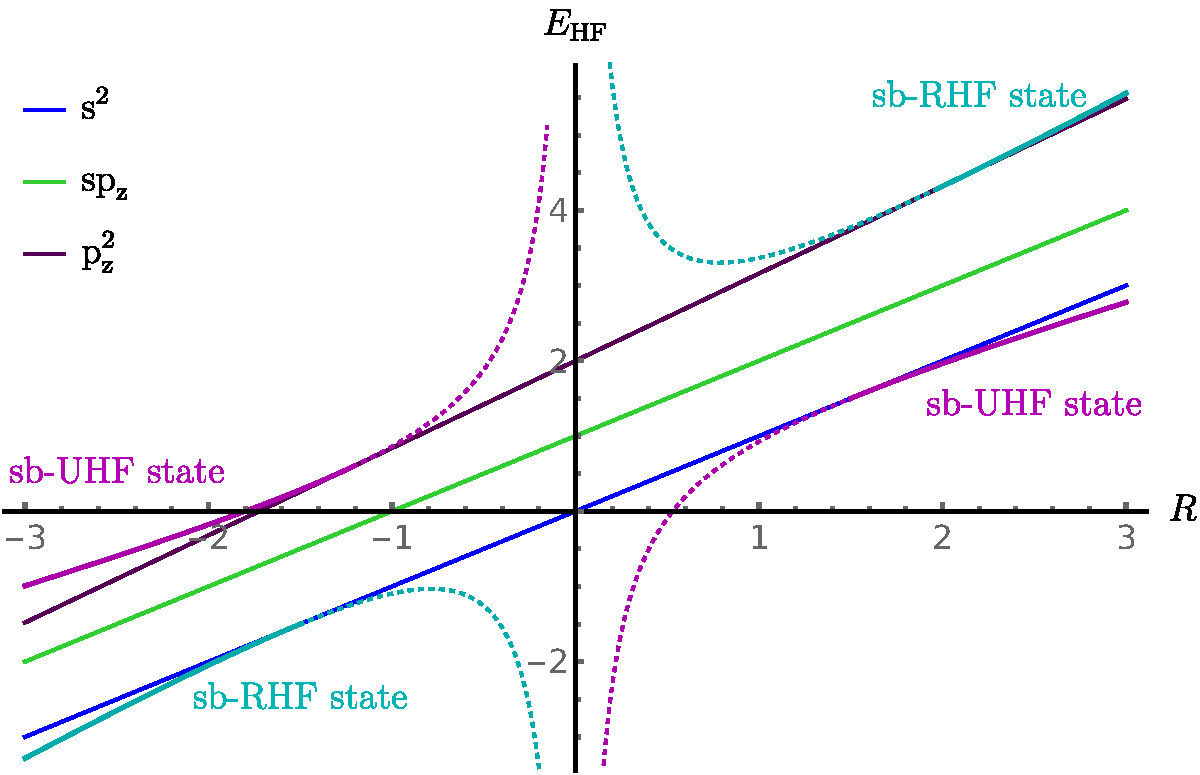
\includegraphics[width=0.9\textwidth]{EsbHF.pdf}
    \caption{\centering Energies of the five solutions of the HF equations (multiplied by $R^2$). The dotted curves correspond to the analytic continuation of the symmetry-broken solutions.}
    \label{fig:SpheriumNrj}
\end{figure}

\section{Radius of convergence and exceptional points}

\subsection{Evolution of the radius of convergence}

In this part, we will try to investigate how some parameters of $\bH(\lambda)$ influence the radius of convergence of the perturbation series. The radius of convergence is equal to the distance of the closest singularity to the origin of $E(\lambda)$. Hence we need to determine the locations of the exceptional points to obtain information on the convergence properties. To find them we solve simultaneously the equations \eqref{eq:PolChar} and \eqref{eq:DPolChar}. The equation \eqref{eq:PolChar} is the well-known secular equation giving the energies of the system, if an energy is also solution of \eqref{eq:DPolChar} then this energy is degenerate. In this case the energies obtained are dependent of $\lambda$ so solving those equations with respect to $E$ and $\lambda$ gives the value of $\lambda$ where two energies are degenerate i.e. the exceptional points.

\begin{equation}\label{eq:PolChar}
\text{det}[E-\bH(\lambda)]=0
\end{equation}

\begin{equation}\label{eq:DPolChar}
\pdv{E}\text{det}[E-\bH(\lambda)]=0
\end{equation}

The electron 1 have a spin $\alpha$ and the electron 2 a spin $\beta$. Hence we can forget the spin part of the spin-orbitals and from now on we will work with spatial orbitals. In the restricted formalism the spatial orbitals are the same so the two-electron basis set is defined as:

\begin{align}\label{eq:rhfbasis}
 \psi_1 & =Y_{00}(\theta_1)Y_{00}(\theta_2),
 & 
 \psi_2 & =Y_{00}(\theta_1)Y_{10}(\theta_2),\\
 \psi_3 & =Y_{10}(\theta_1)Y_{00}(\theta_2),
 & 
 \psi_4 & =Y_{10}(\theta_1)Y_{10}(\theta_2).
\end{align}

The Hamiltonian $\bH(\lambda)$ is block diagonal because of the symmetry of the basis set i.e. $\psi_1$ only interacts with $\psi_4$ and $\psi_2$ with $\psi_3$. The two singly excited states give a singlet sp\textsubscript{z} and a triplet sp\textsubscript{z} state but their symmetry is not the same as the ground state. Thus these states can not be involved in an avoided crossing with the ground state as it can be seen in \autoref{fig:RHFMiniBas} and a fortiori can not be involved in an exceptional point with the ground state. However there is an avoided crossing between the s\textsuperscript{2} state and the p\textsubscript{z}\textsuperscript{2} one which gives two exceptional points in the complex plane. 

\begin{figure}[h!]
    \centering
    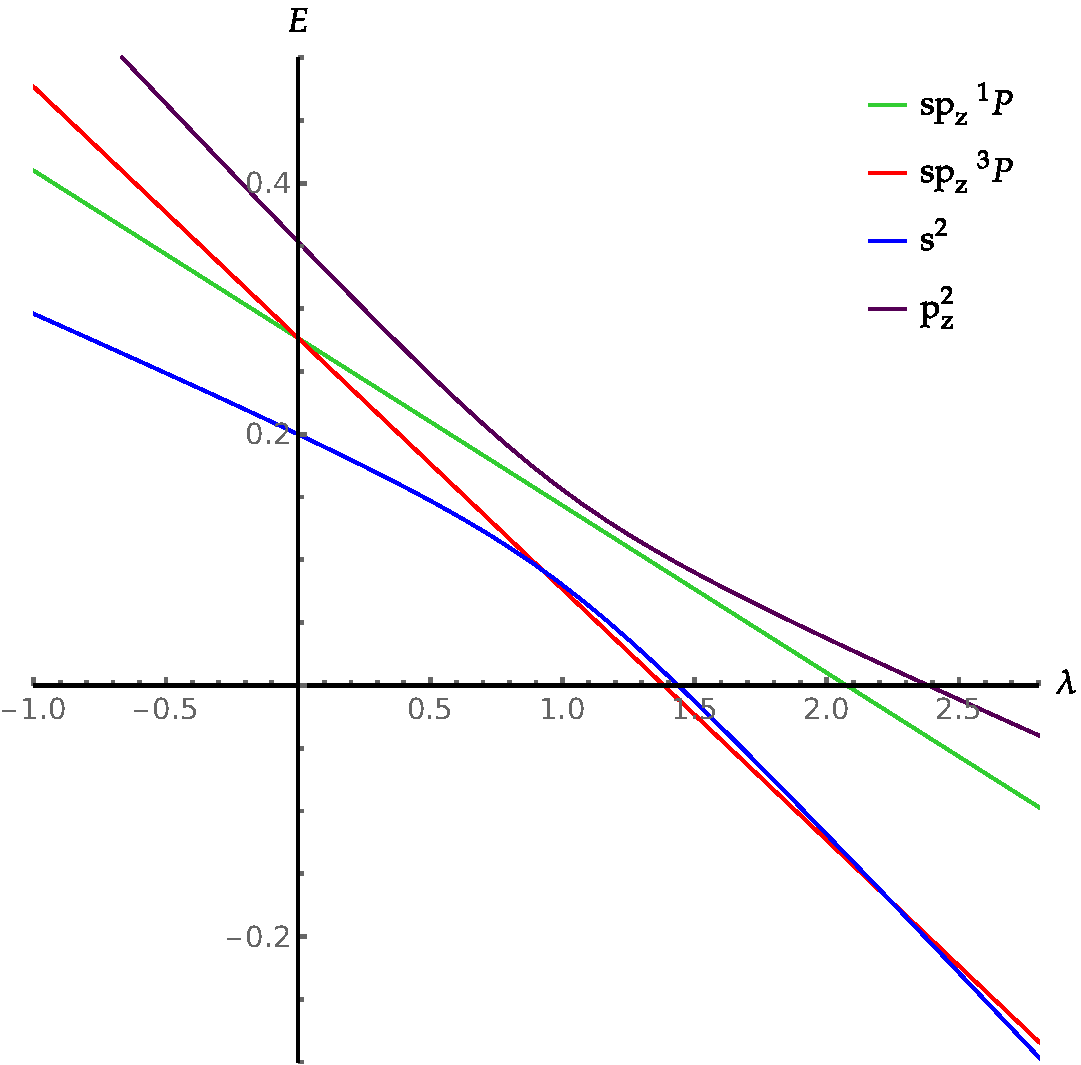
\includegraphics[width=0.7\textwidth]{EMP_RHF_R10.pdf}
    \caption{\centering Energies $E(\lambda)$ in the restricted basis set \eqref{eq:rhfbasis} with $R=10$.}
    \label{fig:RHFMiniBas}
\end{figure}

To simplify the problem, it is convenient to only consider basis functions with the symmetry of the exact wave function, such basis functions are called Configuration State Function (CSF). It simplifies the problem because with such a basis set we only get the degeneracies of interest for the convergence properties i.e. the exceptional points between states with the same symmetry. In this case the ground state is a totally symmetric singlet. According to the angular-momentum theory \cite{AngularBook, SlaterBook, Loos_2009} we expand the exact wave function in the following two-electron basis:
\begin{equation}
\Phi_l(\theta)=\frac{\sqrt{2l+1}}{4\pi R^2}P_l(\cos\theta)
\end{equation}
where $P_l$ are the Legendre polynomial and $\theta$ is the interelectronic angle.

Then using this basis set we can compare the different partitioning of \autoref{sec:AlterPart}. \autoref{fig:RadiusPartitioning} shows the evolution of the radius of convergence $R_{\text{CV}}$ in function of $R$ for the MP, the EN, the Weak Correlation and the Strong Coupling partitioning in a minimal basis i.e. $P_0$ and $P_1$ and in the same basis augmented with $P_2$. We see that the radius of convergence of the strong coupling partitioning is growing with R whereas it is decreasing for the three others partitioning. This result was expected because the three decreasing partitioning use a weakly correlated reference so $\bH^{(0)}$ is a good approximation for small $R$. On the contrary, the strong coupling one uses a strongly correlated reference so this series converge better when the electron are strongly correlated i.e. when $R$ is large for the spherium model.
The MP partitioning is always better than the weak correlation in \autoref{fig:RadiusPartitioning}. In the weak correlation partitioning the powers of $R$ are well-separated so each term of the series is a different power of $R$. Whereas the MP reference is proportionnal to $R^{-1}$ and $R^{-2}$ so the MP series is not well-defined in terms of powers of $R$. Moreover it can be proved that the $n$-th order energy of the weak correlation series can be obtained as a  Taylor approximation of MP$n$ respective to $R$. It seems that the EN partitioning is better than the MP one for very small R in the minimal basis. In fact, it is just an artifact of the minimal basis because in the minimal basis augmented with $P_2
$ (and in larger basis set) the MP series has a greater radius of convergence for all value of $R$.

\begin{figure}[h!]
    \centering
    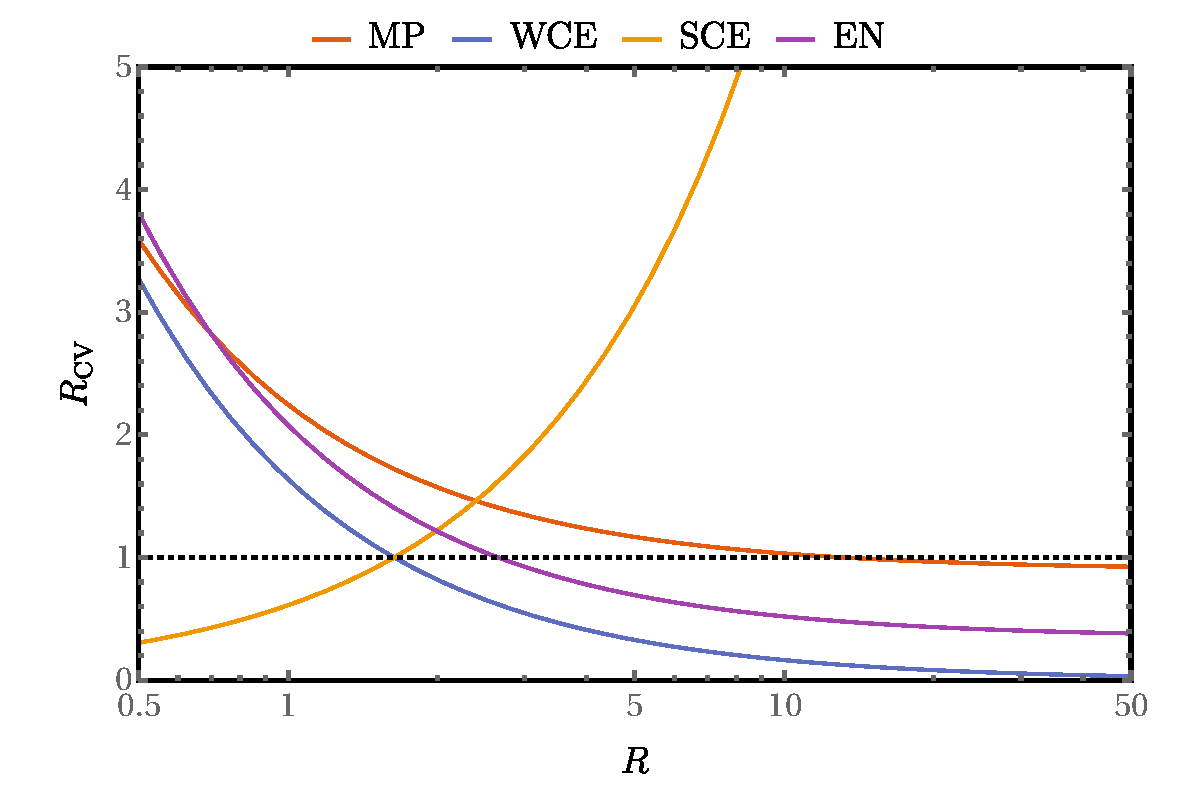
\includegraphics[width=0.45\textwidth]{PartitioningRCV2.pdf}
    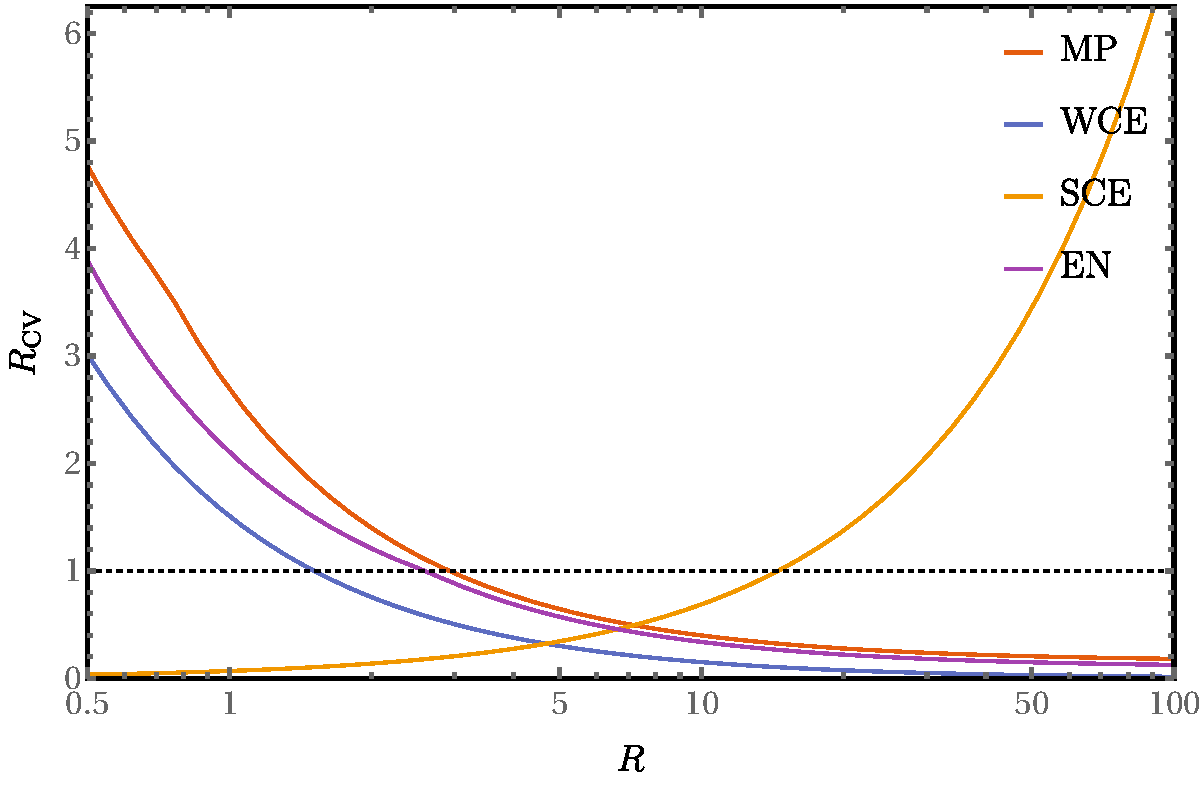
\includegraphics[width=0.45\textwidth]{PartitioningRCV3.pdf}
    \caption{\centering Radius of convergence in the minimal basis (left) and in the minimal basis augmented with $P_2$ (right) for different partitioning of the Hamiltonian $\bH(\lambda)$.}
    \label{fig:RadiusPartitioning}
\end{figure}

\autoref{fig:RadiusBasis} shows that the radius of convergence is not very sensitive to the expansion of the basis set. The CSF basis function have all the same spin and spatial symmetry so we expect that the singularities obtained within this basis set will be $\alpha$ singularities. The \autoref{tab:SingAlpha} proves that the singularities considered in this case are $\alpha$ singularities. This is consistent with the observation of Goodson and Sergeev \cite{Goodson_2004} on $\alpha$ singularities. The discontinuities observed in \autoref{fig:RadiusBasis} with the MP partitioning are due to a change of the dominant singularity. We can observe this change in \autoref{tab:SingAlpha}, the value for $R=1$ and $R=2$ are respectively in the positive and negative plane.

\begin{figure}[h!]
    \centering
    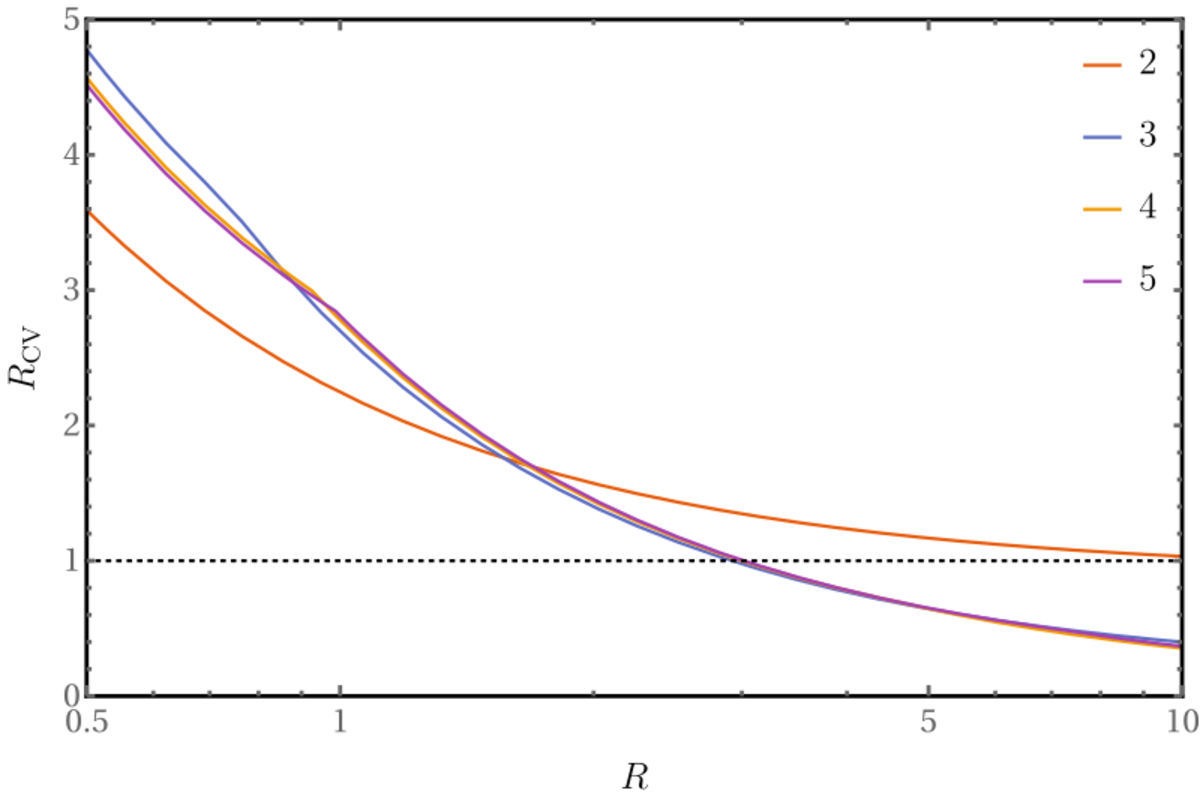
\includegraphics[width=0.45\textwidth]{MPlargebasis.pdf}
    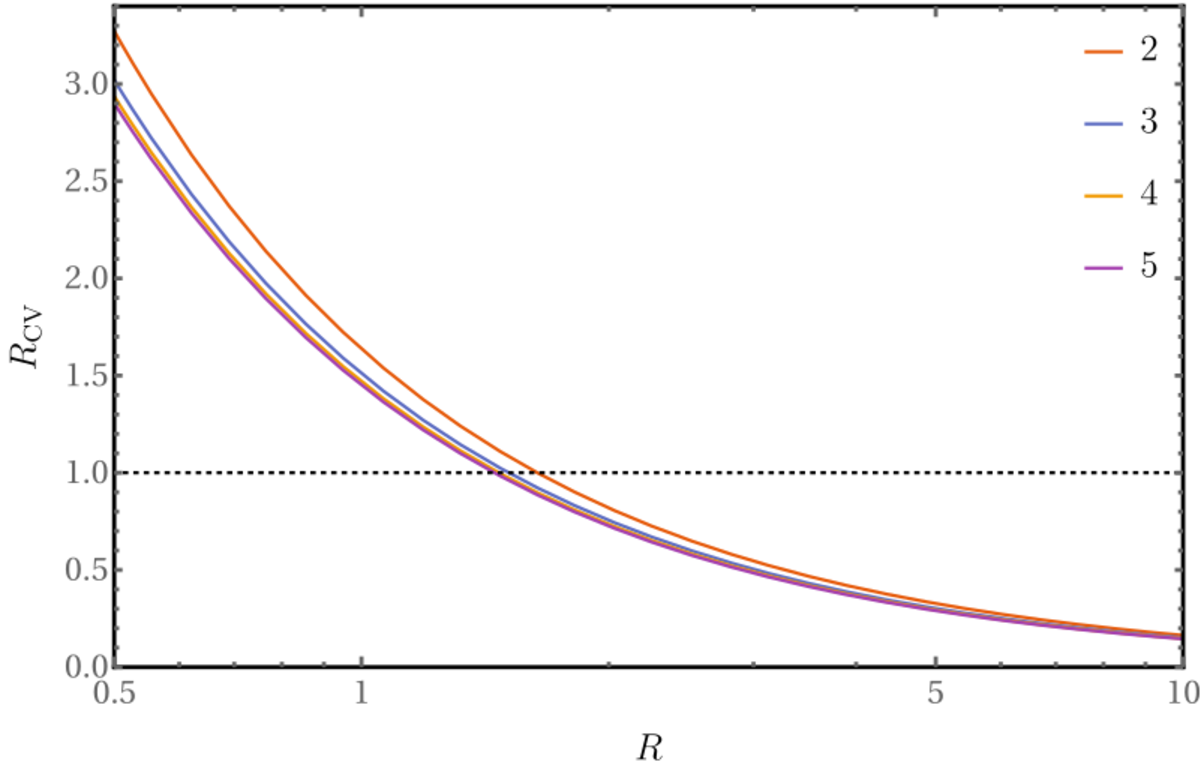
\includegraphics[width=0.45\textwidth]{WCElargebasis.pdf}
    \caption{\centering Radius of convergence in the CSF basis with $K$ basis function for the MP partitioning (left) and the WC partitioning (right).}
    \label{fig:RadiusBasis}
\end{figure}

\begin{table}[h!]
\centering
\caption{\centering Dominant singularity in the CSF basis set ($n=8$) for various value of R. The first line is the value for the MP partitioning and the second for the WC one.}
\begin{tabular}{cccccccc}
\hline
\hline
$R$ & 0.1 & 1 & 2 & 3 & 5 & 10 & 100 \\
\hline
MP & 14.1-10.9i & 2.38-1.47i & -0.67-1.30i & -0.49-0.89i & -0.33-0.55i & -0.22-0.31i & 0.03-0.05i \\
WC & -9.6-10.7i & -0.96-1.07i & -0.48-0.53i & -0.32-0.36 & -0.19-0.21i & -0.10-0.11i & -0.01-0.01i \\
\hline
\hline
\end{tabular}
\label{tab:SingAlpha}
\end{table}

Now we will investigate the differences in the singularity structure between the RHF and UHF formalism. To do this we use the symmetry-broken orbitals obtained in \autoref{sec:spherium}. Thus the UHF two-electron basis is:
\begin{align}\label{eq:uhfbasis}
 \psi_1 & =\phi_{\alpha,1}(\theta_1)\phi_{\beta,1}(\theta_2),
 & 
 \psi_2 & =\phi_{\alpha,1}(\theta_1)\phi_{\beta,2}(\theta_2),\\
 \psi_3 & =\phi_{\alpha,2}(\theta_1)\phi_{\beta,1}(\theta_2),
 & 
 \psi_4 & =\phi_{\alpha,2}(\theta_1)\phi_{\beta,2}(\theta_2).
\end{align}
with the symmetry-broken orbitals
\begin{align*}\label{eq:uhforbitals}
 \phi_{\alpha,1}(\theta) & =\frac{\sqrt{75+62R}Y_{00}(\theta)+5\sqrt{-3+2R}Y_{10}(\theta)}{4\sqrt{7R}},
 & 
 \phi_{\beta,1}(\theta) & =\frac{\sqrt{75+62R}Y_{00}(\theta)-5\sqrt{-3+2R}Y_{10}(\theta)}{4\sqrt{7R}},\\
 \phi_{\alpha,2}(\theta) & =\frac{-5\sqrt{-3+2R}Y_{00}(\theta)+\sqrt{75+62R}Y_{10}(\theta)}{4\sqrt{7R}},
 & 
 \phi_{\beta,2}(\theta) & =\frac{5\sqrt{-3+2R}Y_{00}(\theta)+\sqrt{75+62R}Y_{10}(\theta)}{4\sqrt{7R}}.
\end{align*}

In the UHF formalism the Hamiltonian $\bH(\lambda)$ is no more block diagonal, $\psi_4$ can interact with $\psi_2$ and $\psi_3$. The matrix elements $H_{ij}$ for this interaction are given in \eqref{eq:MatrixElem}. For $R=3/2$ the Hamitonian is block diagonal and this is equivalent to the RHF case but for R>3/2 the matrix elements become real. This interaction corresponds to the spin contamination of the wave function. For $R<3/2$ the matrix elements are complex, this corresponds to the holomorphic solution of \autoref{fig:SpheriumNrj}, the singularities in this case will be treated in \autoref{sec:uhfSing}. The matrix elements become real again for $R<-75/62$, this corresponds to the sb-UHF solution for negative value of $R$ observed in \autoref{sec:spherium}. We will refer to the domain where the matrix element are complex as the holomorphic domain.

\begin{equation}\label{eq:MatrixElem}
H_{24}=H_{34}=H_{42}=H_{43}=\sqrt{-3+2R}\sqrt{75+62R}\frac{25+2R}{280R^3}
\end{equation}

The singularity structure in this case is more complex because of the spin contamination of the wave function. We can not use configuration state function in this case. So when we compute all the degeneracies using \eqref{eq:PolChar} and \eqref{eq:DPolChar} some correspond to EPs and some correspond to conical intersections. The numerical distinction of those singularities is very difficult so we will first look at the energies $E(\lambda)$ obtained with this basis set.
\autoref{fig:UHFMiniBas} is the analog of \autoref{fig:RHFMiniBas} in the UHF formalism. We see that in this case the sp\textsubscript{z} triplet interacts with the s\textsuperscript{2} and the p\textsubscript{z}\textsuperscript{2} singlets. Those avoided crossings are due to the spin contamination of the wave function. The exceptional points resulting from those avoided crossings will be discussed in \autoref{sec:uhfSing}. \\

\begin{figure}[h!]
    \centering
    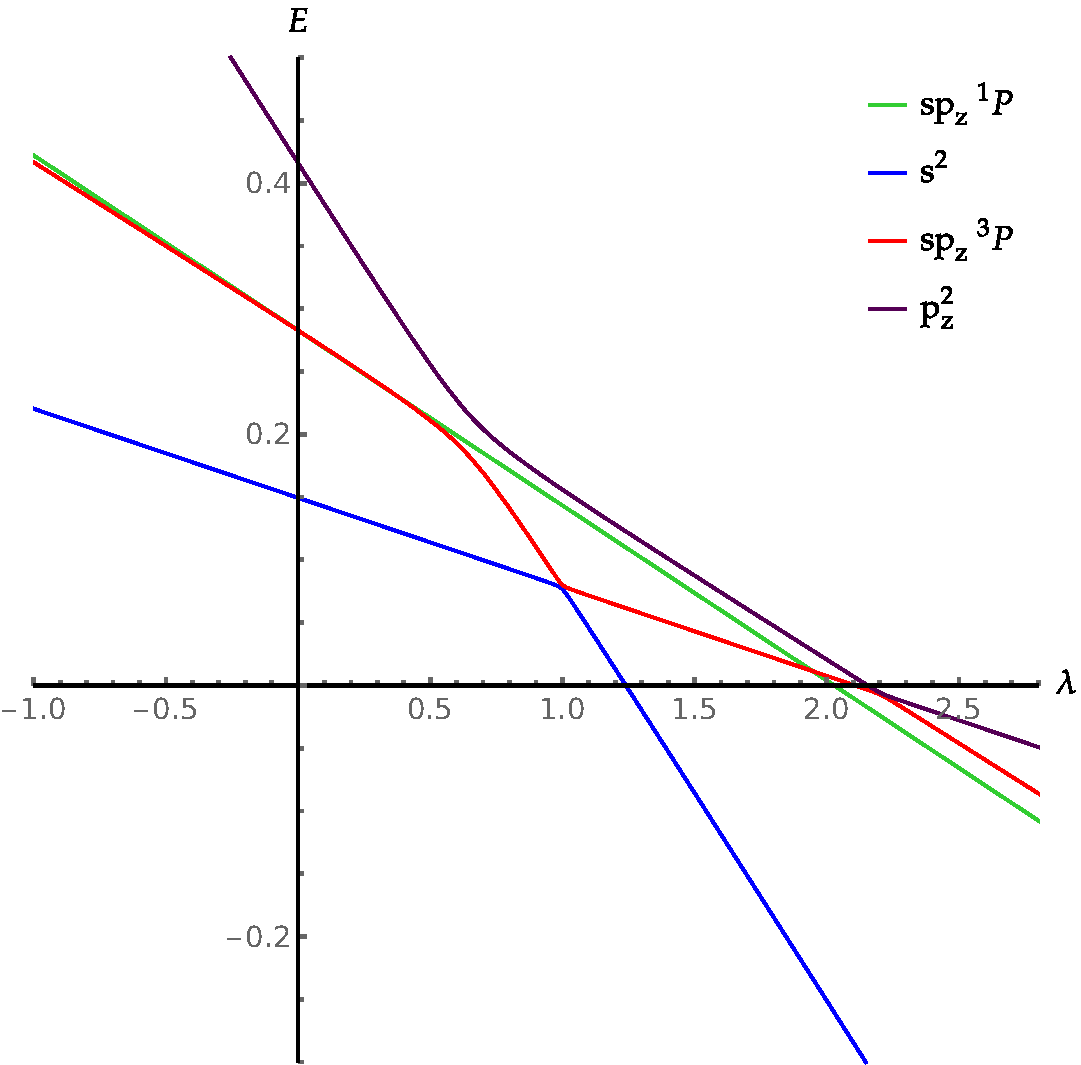
\includegraphics[width=0.7\textwidth]{EMP_UHF_R10.pdf}
    \caption{\centering Energies $E(\lambda)$ in the unrestricted basis set \eqref{eq:uhfbasis} with $R=10$.}
    \label{fig:UHFMiniBas}
\end{figure}

In this study we have used spherical harmonics (or combination of spherical harmonics) as basis function which are diffuse wave functions. It would also be interesting to investigate the use of localized basis function \cite{Seidl_2018} (for example gaussians) because those functions would be more adapted to describe the correlated regime. \\

\subsection{Exceptional points in the UHF formalism}\label{sec:uhfSing}

In the RHF case there are only $\alpha$ singularities and large avoided crossings but we can see in \autoref{fig:UHFMiniBas} that in the UHF case there are sharp avoided crossings which are connected to $\beta$ singularities. For example at $R=10$ the pair of singularities connected to the avoided crossing between s\textsuperscript{2} and sp\textsubscript{z} $^{3}P$ is $0.999\pm0.014i$. And the one between sp\textsubscript{z} $^{3}P$ and p\textsubscript{z}\textsuperscript{2} is connected with the singularities $2.207\pm0.023i$. However in the spherium the electrons can't be ionized so those singularities are not the $\beta$ singularities highlighted by Sergeev and Goodson \cite{Sergeev_2005}. We can see in \autoref{fig:UHFEP} that the degeneracy between the s\textsuperscript{2} singlet and the sp\textsubscript{z} triplet at $R=3/2$. For $R>3/2$, it becomes an avoided crossing on the real axis and the degeneracies are moved in the complex plane. The wave function is spin contaminated for $R>3/2$ this why the s\textsuperscript{2} singlet energy can not cross the sp\textsubscript{z} triplet curves anymore. When $R$ increases this avoided crossing becomes sharper. As presented before $\beta$ singularities are linked to quantum phase transition so it seems that this singularity is linked to the spin symmetry breaking of the UHF wave function. The fact that a similar pair of $\beta$ singularities appears for $R<-75/62$ confirms this assumption. A second pair of $\beta$ singularities appear for $R\gtrsim 2.5$, this is probably due to an excited-state quantum phase transition but this still need to be investigated. 

\begin{figure}[h!]
    \centering
    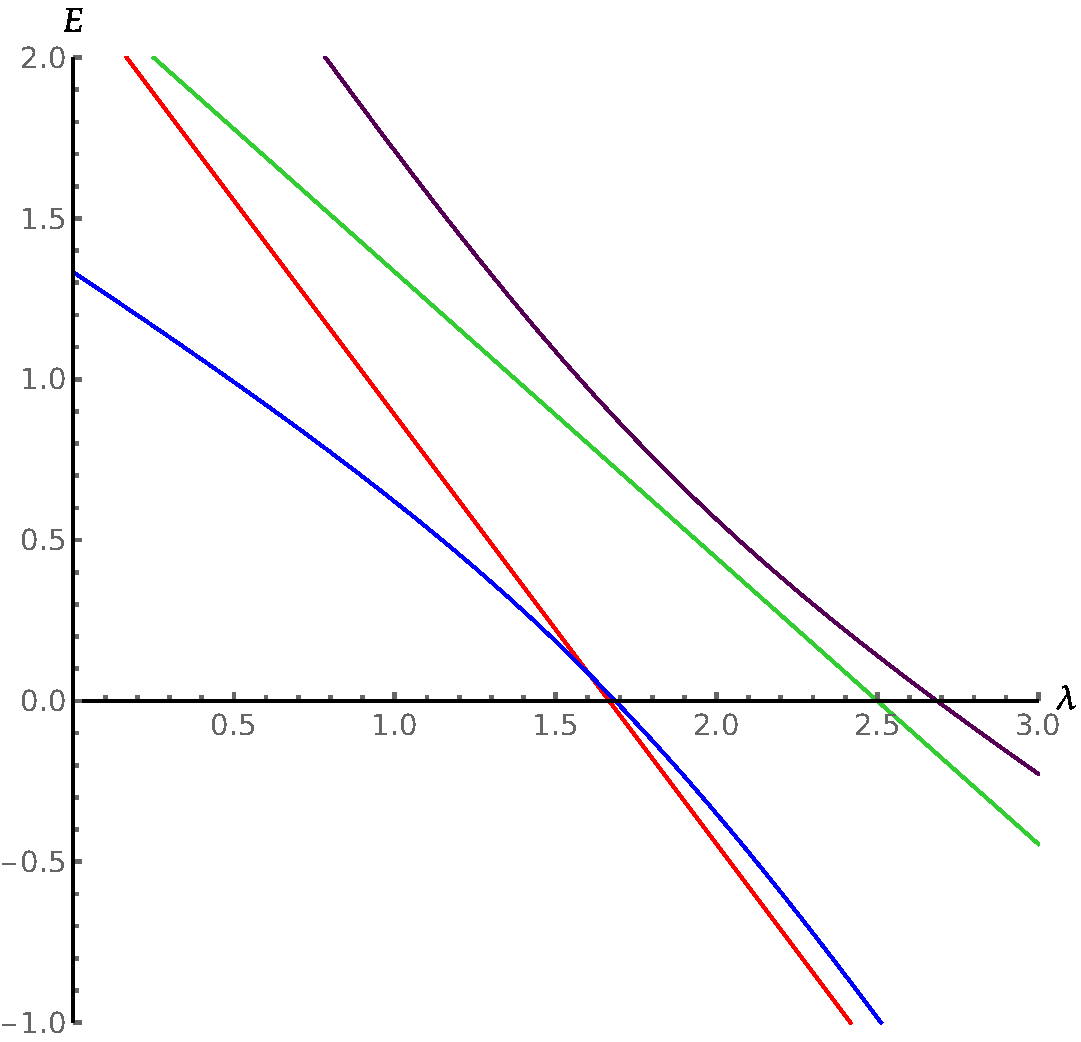
\includegraphics[width=0.45\textwidth]{UHFCI.pdf}
    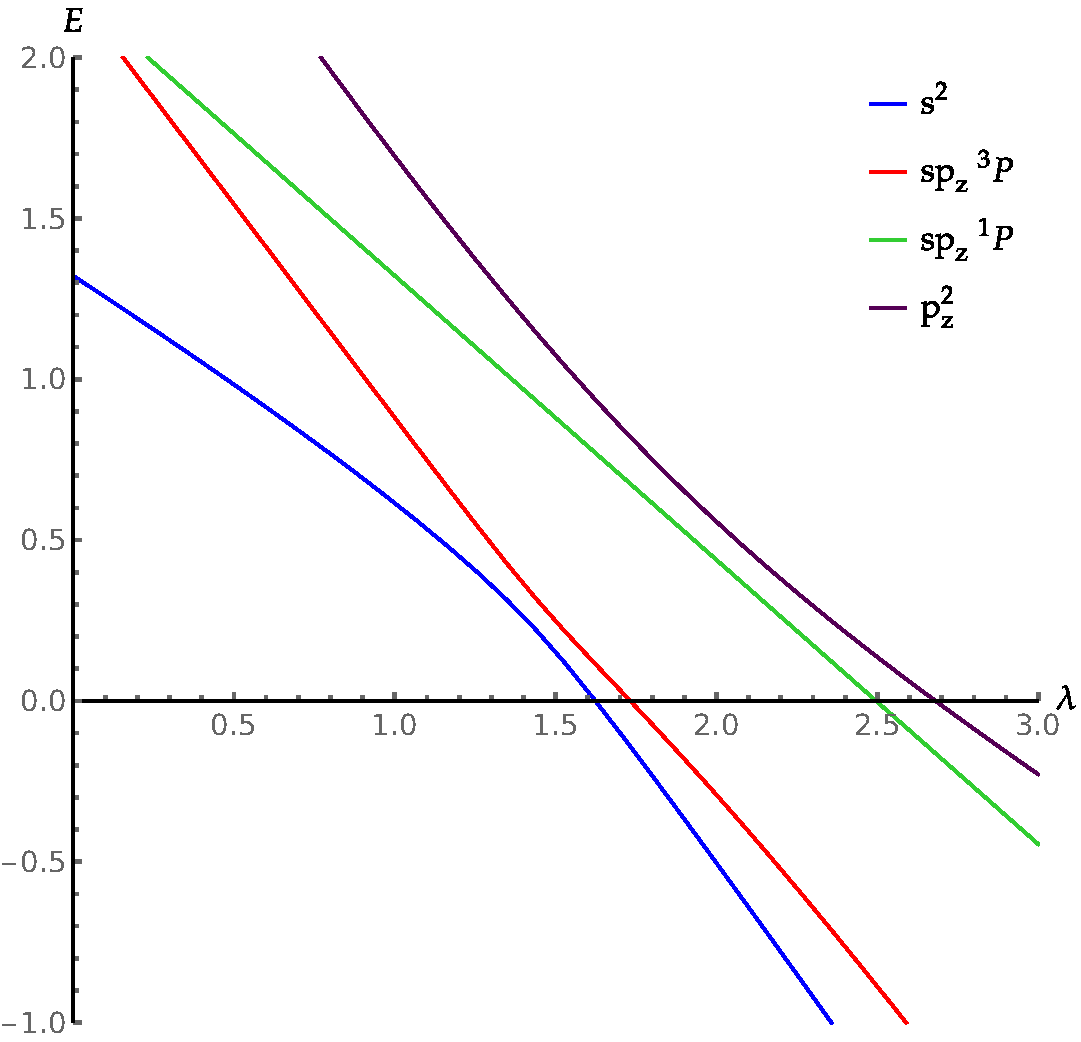
\includegraphics[width=0.45\textwidth]{UHFEP.pdf}
    \caption{\centering Energies $E(\lambda)$ in the unrestricted basis set \eqref{eq:uhfbasis} for $R=1.5$ (left) and $R=1.51$ (right).}
    \label{fig:UHFEP}
\end{figure}

As shown before, some matrix elements of the Hamiltonian become complex in the holomorphic domain. Therefore the Hamiltonian becomes non-Hermitian for those value of $R$. In \cite{Burton_2019a} Burton et al. proved that for the \ce{H_2} molecule the unrestricted Hamiltonian is not \pt -symmetric in the holomorphic domain. An analog reasoning can be done with the spherium model to prove the same result. The \pt -symmetry (invariance with respect to combined space reflection $\mathcal{P}$ and time reversal $\mathcal{T}$) is a property which ensures that a non-Hermitian Hamiltonian has a real energy spectrum. Thus \pt -symmetric Hamiltonian can be seen as an intermediate between Hermitian and non-Hermitian.

\autoref{fig:UHFPT} shows that for the spherium model a part of the energy spectrum becomes complex when R is in the holomorphic domain. The parameter domain of value where the energy becomes complex is called the broken \pt symmetry  region. This is consistent with the fact that in the holomorphic domain the Hamiltonian break the \pt -symmetry. 

\begin{figure}[h!]
    \centering
    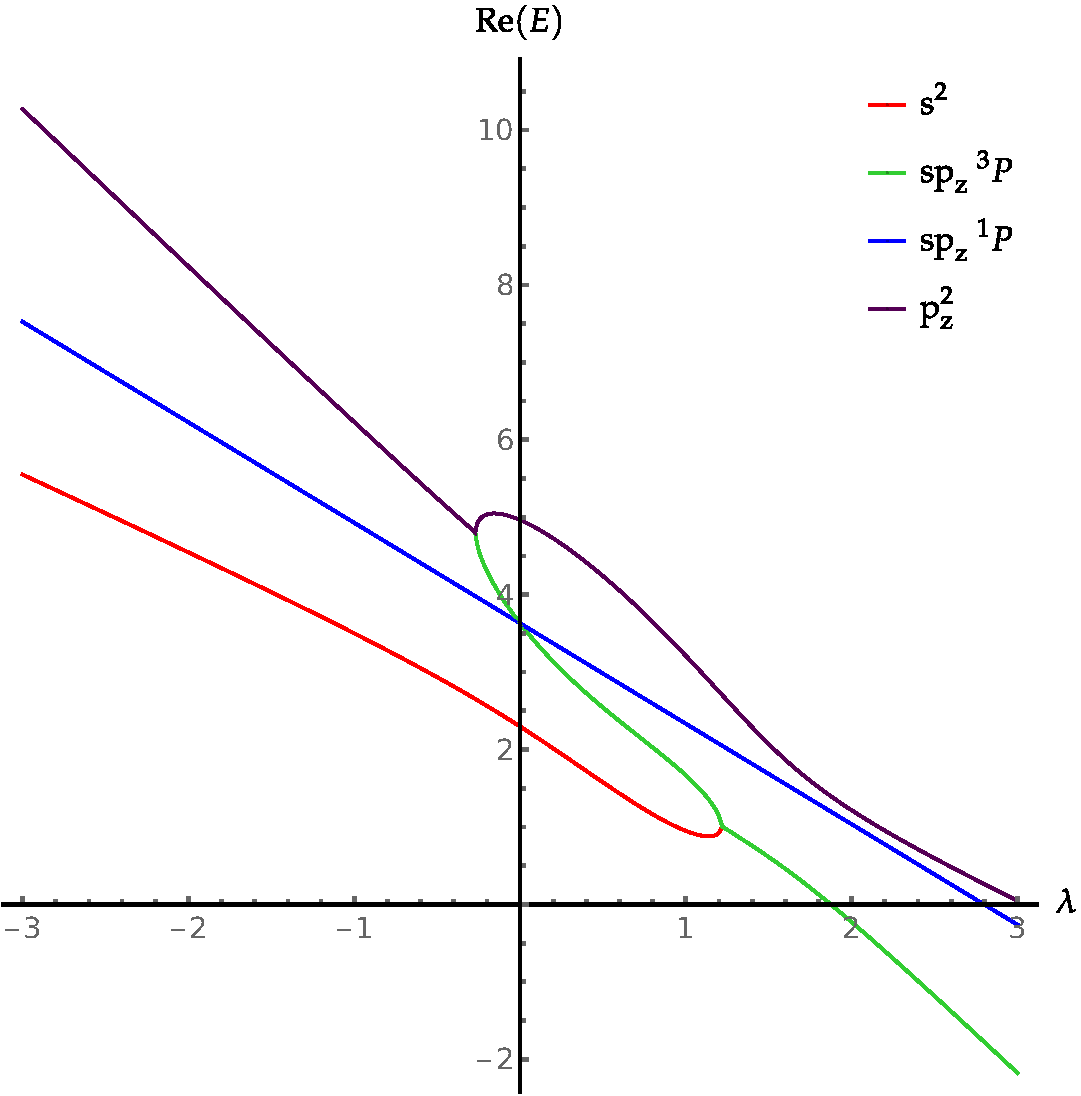
\includegraphics[width=0.45\textwidth]{ReNRJPT.pdf}
    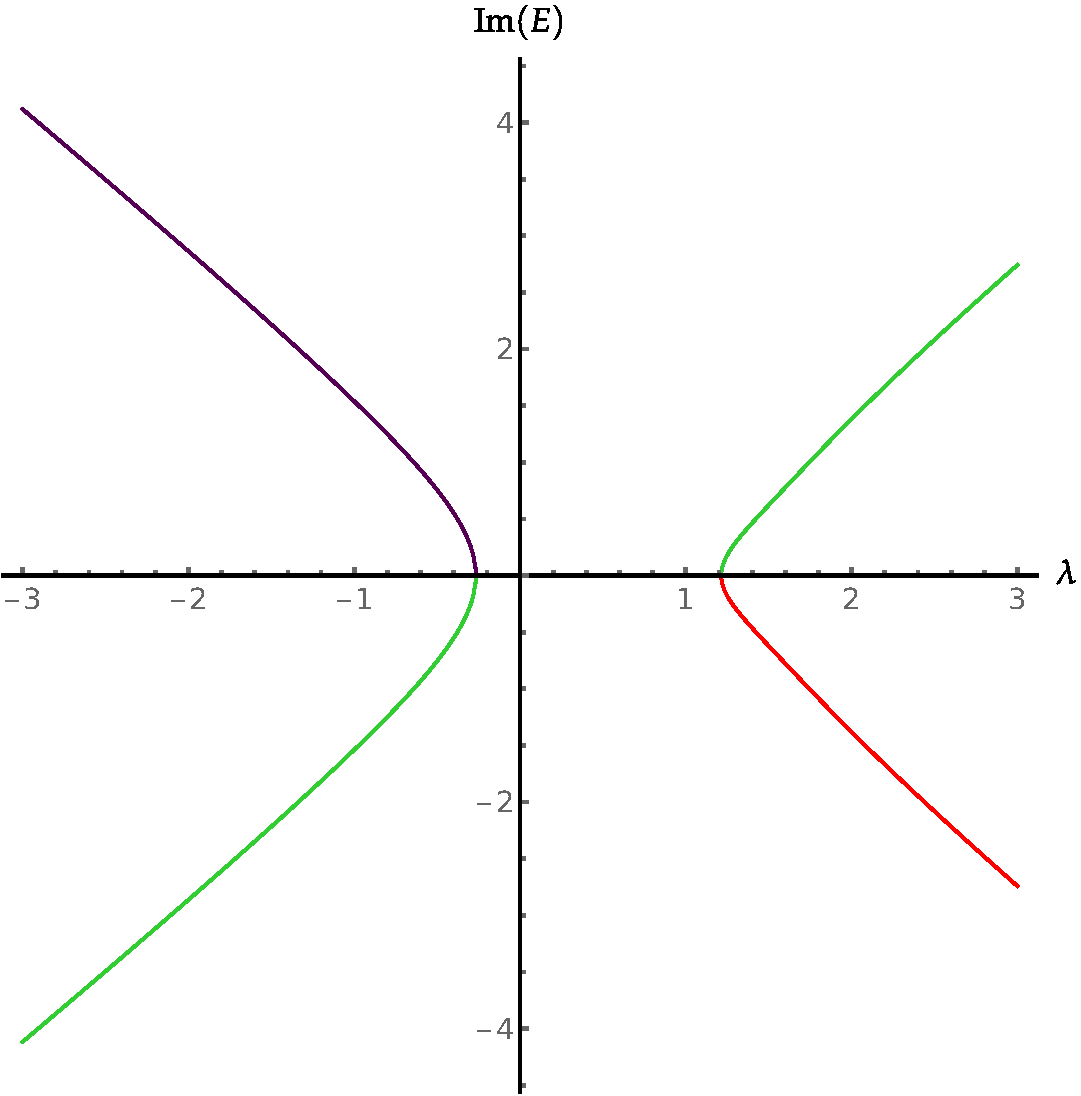
\includegraphics[width=0.45\textwidth]{ImNRJPT.pdf}
    \caption{\centering Real part (left) and imaginary part (right) of $E(\lambda)$ in the unrestricted basis set \eqref{eq:uhfbasis} for $R=1$.}
    \label{fig:UHFPT}
\end{figure}

For a non-Hermitian Hamiltonian the exceptional points can lie on the real axis. In particular, at the point of PT transition (the point where the energies become complex) the two energies are degenerate resulting in such an exceptional point on the real axis. This degeneracy can be seen in \autoref{fig:UHFPT}.

\section{Conclusion}


\newpage
\printbibliography

\newpage
\appendix

\section{ERHF and EUHF}

\end{document}
